% !TEX program=pdflatex
% LaTeX rebuttal letter example. 
% 
% Copyright 2019 Friedemann Zenke, fzenke.net
%
% Based on examples by Dirk Eddelbuettel, Fran and others from 
% https://tex.stackexchange.com/questions/2317/latex-style-or-macro-for-detailed-response-to-referee-report
% 
% Licensed under cc by-sa 3.0 with attribution required.

\documentclass[12pt]{article}
\usepackage[utf8]{inputenc}
\usepackage{lipsum} % to generate some filler text
\usepackage{fullpage}
\usepackage{times}
\usepackage{amsmath, amsthm, amsfonts}
\usepackage{booktabs}
\usepackage{makecell}
\usepackage{multirow}
\usepackage{lscape}
\usepackage{xcolor}
\usepackage{float}
\usepackage{subfig}
\usepackage{graphicx}
\usepackage{framed}
\usepackage{soul}
\usepackage[colorlinks=true, linkcolor=blue]{hyperref}
% Vector
\newcommand{\MyVec}[1]{\boldsymbol{#1}}
% Matrix
\newcommand{\MyMat}[1]{\boldsymbol{#1}}
% Vectors with hat
\newcommand{\hvec}[1]{\hat{\boldsymbol{h}}_{#1}}
% Model parameters
\newcommand{\Param}[1]{\textcolor{blue}{#1}}

\usepackage{blindtext}
\usepackage[most]{tcolorbox} 
\definecolor{block-gray}{gray}{0.95}


\newtcolorbox{zitat}[2][]{%
    colback=block-gray,
    grow to right by=-0mm,
    grow to left by=-0mm, 
    boxrule=0pt,
    boxsep=0pt,
    breakable,
    enhanced jigsaw,
    borderline west={4pt}{0pt}{gray},
    title={#2\par},
    colbacktitle={block-gray},
    coltitle={black},
    fonttitle={\bfseries},
    attach title to upper={},
    #1,
}

\newenvironment{myquote}[1]%
{\vspace{0.5em}\begin{zitat}{#1}}
{\end{zitat}\vspace{0.5em}}


% import Eq and Section references from the main manuscript where needed
% \usepackage{xr}
% \externaldocument{manuscript}

% package needed for optional arguments
\usepackage{xifthen}
% define counters for reviewers and their points
\newcounter{reviewer}
\setcounter{reviewer}{0}
\newcounter{point}[reviewer]
\setcounter{point}{0}

% This refines the format of how the reviewer/point reference will appear.
\renewcommand{\thepoint}{P\,\thereviewer.\arabic{point}} 

% command declarations for reviewer points and our responses
\newcommand{\reviewersection}{\stepcounter{reviewer} \bigskip \hrule
                  \section*{Reviewer \thereviewer}}

\newenvironment{point}
   {\refstepcounter{point} \bigskip \noindent {\textbf{Reviewer~Point~\thepoint} } ---\ \begin{sf}}
   {\end{sf} \par}

\newcommand{\shortpoint}[1]{\refstepcounter{point}  \bigskip \noindent 
	{\textbf{Reviewer~Point~\thepoint} } ---\begin{sf} ~#1 \end{sf}\par}

\newenvironment{reply}
   {\medskip \noindent \textbf{Reply}:\  }
   {\medskip}

\newcommand{\shortreply}[2][]{\medskip \noindent \textbf{Reply}:\  #2
	\ifthenelse{\equal{#1}{}}{}{ \hfill \footnotesize (#1)}%
	\medskip}

\begin{document}

\section*{Response to the Reviewers}
% General intro text goes here
We thank the reviewers for their critical assessment and insightful comments of our work.
%
We have made extensive modifications to our manuscript.
%
In the following we address their concerns point by point.
%
We also prepare an \emph{annotated version} for our revised manuscript.
%
In the annotated version, changes corresponding to each point are all highlighted by red squares.

\subsection*{Summary of Changes}

TODO

% Let's start point-by-point with Reviewer 1
\reviewersection

% R1Q0
\begin{point}
    The authors conduct an empirical analysis of performance bottlenecks in graph neural network training. The authors identify the edge-related calculation is the performance bottleneck. Experimental of several GNN variants, such as GCN, GGNNNN, GAT and GaAN on six real-world graph datasets verify the importance of the findings. The experimental analysis is sufficient. However, there are some tiny issues in this paper.
\end{point}

\begin{reply}
    Thank you for your kindly comments on our manuscript.
    %
    We have carefully revised the manuscript according to your suggestions. 
    %
    Please see the replies below.
    %
    The changes corresponding to each point are highlighted by red squares in the annotated version of our revised manuscript.

\end{reply}

% R1Q1
\begin{point}
	There are lots of symbols in this paper. Some symbols are reused and confusing, such as s denotes sub-layers or edge features.
\end{point}

% Our reply
\begin{reply}
    We apologize for the confusing use of symbols.
    %
    To clarify the symbol usage, we have checked our manuscript and unified the usage of symbol in the revised version.
    %
    After revision, each symbol only represents one meaning.
    %
    We added Table 1 at the beginning of Section 2 ``Review of Graph Neural Networks'' in the revised version to summarize frequently-used symbols.
    %
    We quote the table below:
    \begin{table}[H]
        \footnotesize
        \centering
        \begin{tabular}{p{3em}lp{35em}}
            \toprule
            Category & Symbol & Meaning \\
            \midrule
            \multirow[c]{4}{3em}{Graph Structure}& $\mathcal{G}=(\mathcal{V}, \mathcal{E})$ & The simple undirected input graph with the vertex set $\mathcal{V}$ and the edge set $\mathcal{E}$. \\
            & $v_x$ & The $x$-th vertex of the input graph. \\
            & $e_{y,x}$ & The edge pointing from $v_y$ to $v_x$ of the input graph. \\
            & $\mathcal{N}(v_x)$ & The adjacency set of $v_x$ in the input graph. \\ 
            & $\bar{d}$ & The average degree of the input graph. \\ \midrule
            \multirow[c]{6}{3em}{GNN Definition}& $L$ & The number of GNN layers. \\
            & $K$ & The number of heads in a GNN layer. \\
            & $\phi^l$ & The messaging function of the GNN layer $l$. \\
            & $\Sigma^l$ & The aggregation function of the GNN layer $l$. \\
            & $\gamma^l$ & The vertex updating function of the GNN layer $l$. \\ 
            & $\phi^{l,i}$ / $\Sigma^{l,i}$ / $\gamma^{l,i}$ & The messaging/aggregation/updating function of the $i$-th sub-layer of the GNN layer  $l$.\\
            & $\textcolor{blue}{\boldsymbol{W}^l, \boldsymbol{W}^{(k)}/\boldsymbol{b}, \boldsymbol{a}}$ & The matrices/vectors represented by the blue characters are the weight matrices/vectors that need to be learned in the GNN. \\  \midrule
            \multirow[c]{8}{3em}{Vector}& $\boldsymbol{v}_x$ & The feature vector of the vertex $v_x$. \\
            & $\boldsymbol{e}_{y,x}$ & The feature vector of the edge $e_{y,x}$.  \\
            & $\boldsymbol{h}_x^{l}$ &  The {input} hidden vector of the graph neuron corresponding to $v_x$ in the GNN layer $l$. \\
            & $\boldsymbol{h}_x^{l+1}$ &  The {output} hidden vector of the graph neuron corresponding to $v_x$ in the GNN layer $l$.\\
            & $\boldsymbol{m}_{y,x}^l$ & The message vector of the edge $e_{y,x}$ outputted by $\phi^l$ of the GNN layer $l$. \\
            & $\boldsymbol{s}_{x}^l$ & The aggregated vector of the vertex $v_x$ outputted by $\Sigma^l$ of the GNN layer $l$. \\
            & $\boldsymbol{h}_{x}^{l,i}$ / $\boldsymbol{m}_{y,x}^{l,i}$ / $\boldsymbol{s}_{x}^{l,i}$ & The hidden/message/aggregated vector of the vertex $v_x$ outputted by $\gamma^{l,i}$/$\phi^{l,i}$/$\Sigma^{l,i}$ of the $i$-th sub-layer of the GNN layer $l$. \\
            & $d^l_{in}$, $d^l_{out}$ &  The dimension of the input/output hidden vectors of the GNN layer $l$. \\
            & $dim(\MyVec{x})$ & The dimension of a vector $\MyVec{x}$. \\
            \bottomrule
        \end{tabular}
\end{table}

    
    In the revised manuscript, we use $e_{y,x}$ to represent an edge and use $\boldsymbol{e}_{y,x}$ to represent its input feature vector.
    %
    %The input feature vectors of all edges are same for all GNN layers.
    %
    We use $\boldsymbol{s}$ to represent aggregated vectors outputted by the aggregation function $\Sigma$ in graph neurons.
    %
    For every vertex $v_x$, we use $\boldsymbol{s}^l_x$ to denote the aggregated vector in the graph neuron of $v_x$ in the GNN layer $l$.
    %
    If the GNN layer $l$ has sub-layers, $\boldsymbol{s}^{l,i}_x$ represents the aggregated vector of $v_x$ in the $i$-th sub-layer.
    
    To clarify the concept of \emph{sub-layers} in a GNN layer, we have added more description in the revised manuscript.
    %
    We first introduce the concept of sub-layer in Section 2.2 ``Graph Neuron and Message-passing Model'' as:
    %
    \begin{myquote}{Section 2.2 ``Graph Neuron and Message-passing Model''}
        Some complex GNNs like GAT [6] and GaAN [7] use more than one message passing phase in each GNN layer.
        %
        We regard every message passing phase in a GNN layer as a \emph{sub-layer}.
        %
        We will give out more details on sub-layers when we introduce GAT.
    \end{myquote}
    %
    We then use GAT as an example to elaborate on the concept of sub-layers in Section 2.3 ``Representative GNNs'' as:
    %
    \begin{myquote}{Section 2.3.3 ``GAT (Low Vertex \& High Edge Complexity)''}
        \newcommand{\GATCalcWeight}{\exp(LeakyReLU(\Param{\MyVec{a}}^T[\hvec{y}^l[k] \parallel \hvec{x}^l[k]]))}
        Each GAT layer consists of a vertex pre-processing phase and two sub-layers (i.e., message-passing phases).
        
        The vertex pre-processing phase calculates the attention vector $\hat{\boldsymbol{h}}^{l}_{x}$ for every vertex $v_x$ by $\hvec{x}^l = \parallel_{k=1}^K \Param{\MyMat{W}^l_{(k)}}\MyVec{h}^l_x$. We denote the attention sub-vector generated by the $k$-th head as $\hvec{x}^l[k]=\Param{\MyMat{W}^l_{(k)}}\MyVec{h}^l_x$.
        
        The first sub-layer of GAT (defined in Equation~\ref{eq:GAT-sub-layer-1}) uses the attention vectors to emit the attention weight vector $\boldsymbol{m}^{l,0}_{y,x}$ for every edge $e_{y,x}$ and aggregates the attention weight vectors for every vertex $v_x$ to get the weight sum vector $\MyVec{h}^{l,0}_x$.
        %
        \begin{equation}
            \footnotesize
            \label{eq:GAT-sub-layer-1}
            \begin{aligned}
                \MyVec{m}^{l,0}_{y,x} & = \phi^{l,0}(\MyVec{h}^l_y, \MyVec{h}^l_x, \MyVec{e}_{y,x}, \hvec{y}^l, \hvec{x}^l) = \parallel_{k=1}^{K}\GATCalcWeight, \\
                \MyVec{s}^{l,0}_{x} &= {\Sigma}_{v_y \in \mathcal{N}(v_x)}{\MyVec{m}^{l,0}_{y,x}}, \\
                \MyVec{h}^{l,0}_{x} &= \gamma^{l,0}(\MyVec{h}^l_x, \MyVec{s}^{l,0}_{x})  = \MyVec{s}^{l,0}_{x}.
            \end{aligned}
        \end{equation}
        %
        The second sub-layer of GAT (defined in Equation~\ref{eq:GAT-sub-layer-2}) uses the weight sum vectors to normalize the attention weights for every edge and aggregates the attention vectors $\boldsymbol{\hat{h}}^l_y$ with the normalized weights.
        %
        The aggregated attention vectors $\MyVec{s}^{l,1}_x$ are transformed by an activation function $\delta$ and are outputted as the hidden vectors of the current layer $\MyVec{h}^{l+1}_x$.
        %
        \begin{equation}
            \footnotesize
            \label{eq:GAT-sub-layer-2}
            \begin{aligned}
                \MyVec{m}^{l,1}_{y,x} &= \phi^{l,1}(\MyVec{h}^{l,0}_y, \MyVec{h}^{l,0}_x, \MyVec{e}_{y,x}, \hvec{y}^l, \hvec{x}^l) = \parallel_{k=1}^{K}\frac{\GATCalcWeight}{\MyVec{h}^{l,0}_x[k]}\hvec{y}^l[k], \\
                \MyVec{s}^{l,1}_x &= {\Sigma}_{v_y \in \mathcal{N}(v_x)} \MyVec{m}^{l,1}_{y,x}, \\
                \MyVec{h}^{l+1}_x = \MyVec{h}^{l,1}_x &= \gamma^{l,1}(\MyVec{h}^{l,0}, \MyVec{s}^{l,1}_x) = \delta(\MyVec{s}^{l,1}_x).
            \end{aligned}
        \end{equation}
    \end{myquote}
\end{reply}

% R1Q2
\begin{point}
    Some typical applications of GNNs should be included, such as video object segmentation [ref1], human-object interaction [ref2] and human-parsing [ref3].[1] Zero-shot video object segmentation via attentive graph neural networks,iccv 2019 [2] Learning human-object interactions by graph parsing neural networks, eccv 2018. [3] Hierarchical human parsing with typed part-relation reasoning, cvpr 2020.
\end{point}

\begin{reply}
	Thank you for pointing out missing references. Computer vision is indeed an important application area of graph neural networks. We have added the mentioned references in Section 1 ``Introduction'' in the revised manuscript. We quote the related sentence below:
    \begin{myquote}{Section 1 ``Introduction''}
         The powerful expression ability makes GNNs achieve good accuracy in not only graph analytical tasks [8, 9, 10] (like node classification and link prediction) but also computer vision tasks (like human-object interaction [11], human parsing [12], and video object segmentation [13]).
    \end{myquote}
\end{reply}

% R1Q3
\begin{point}
There are some grammar errors and typos:
\\
  - `Take the demo GNN in Figure 1(a) as  the example.'
\\
 - `to calculate the  output hidden vector $h^{l+1}$ of the current layer l, i.e., $h^{l+1}$ = $\gamma^l(h^l,s^l)$ The end-to-end training requires…'
\\
 - `Implementing it with the specially optimized basic operators on the GPU is a potential optimization'
\\
 - The sentences in the experimental section should be unified.
\end{point}

\begin{reply}

    Thank you for pointing them out.
    %
    We feel really sorry for our carelessness.
    %
    We have proofread our revised manuscript carefully to eliminate grammar errors and typos.
    %
    We have also unified the tenses of the sentences in Section 3 ``Evaluation Design'' and Section 4 ``Evaluation Results and Analysis''.
    %
    We use the past tense to describe experimental methods, results and what they indicate.
    %
    We only use the present tense in the sentences that FigureX/Table X are the subjects of the sentences.

\end{reply}

% R1Q4
\begin{point}
    Figures 6 and 7 should be adjusted. The figures and fonts are too small.
\end{point}

\begin{reply}
    
    As you suggested, we have adjusted all the figures (besides Figure 6 and Figure 7) in the revised manuscript to make sure that font sizes in figures are no less than the font size of figure captions.
    %
    To make the figures more easy to read, we also split Figure 6 and Figure 7 into five figures (Figure 6 to 10) in the revised manuscript to enlarge the subfigures.
    
\end{reply}

% R1Q5
\begin{point}
    In my view, computation efficiency is to describe the testing or validation process. Except for reporting and analyzing the training times, it is meaningful to discuss the inference time. This is also an important point of view for deep learning researchers to be concerned about.
\end{point}

\begin{reply}
    Thank you for the insightful comment and suggestion.
    %
    The efficiency of inference (including inference time and memory usage) is indeed important for deep learning researchers and engineers.
    %
    In the revised manuscript, we have added a new subsection (Section 2.5 ``Inference with GNNs'') to briefly review how to perform inference with GNNs.
    %
    We quote the added subsection below.
    
    \begin{myquote}{Section 2.5 ``Inference with GNNs''}
    The model parameters of a GNN consist of the weight vectors/matrices in the prediction layer and the messaging/aggregation/updating functions of each GNN layer.
    %
    For transductive learning, the input graphs of training and inference are same.
    %
    The structure of the GNN does not need to adjust. 
    %
    For inductive learning, the input graphs used in training and inference are different.
    %
    When we want to perform inference on a new graph with a pre-trained GNN, the structure of the GNN needs to be adjusted, but the hyper-parameters and the model parameters of the GNN remain unchanged.
    %
    The number of graph neurons in each GNN layer has to be adjusted to $|\mathcal{V}|$ of the new graph.
    %
    The connections of graph neurons between GNN layers are also adjusted according to the edge set of the new graph.
    %
    During inference, input feature vectors of the input graph are propagated forward from the input layer to the prediction layer to give out predicted labels.
    
    When the memory capacity of the GPU is large enough to hold all of the input graph and intermediate results during inference, the inference can produce predicted labels for all vertices and edges at once, making full use of the computing power of the GPU.
    %
    When the memory capacity is not large enough, the sampling technique must be adopted.
    
    The sample-based inference splits the test set into several batches.
    %
    For each batch, the sample-based inference samples a subgraph related to the batch from the input graph.
    %
    It performs inference on the sampled subgraph to produce predicted labels for the batch.
    %
    Since the sampled subgraph is usually much smaller than the original input graph, the memory usage during inference is limited.
    %
    The sampling method depends on the prediction task.
    %
    Taking the node classification task as an example, if there are $L$ GNN layers in the GNN, the hidden vector outputted by the last GNN layer of each vertex $\MyVec{h}^L_x$ is only related to the $L$-hop neighborhood of $v_x$.
    %
    Thus, if we want to predict labels for a group of vertices, we only need to sample a subgraph that contains $L$-hop neighborhoods of all given vertices.
    
    The implementation of sample-based inference in PyG stores the whole input graph and its feature vectors in the main memory.
    %
    In the node classification task, it splits the vertices in the test set into batches accoding to a given batch size.
    %
    The subgraph corresponding to each batch is sampled on the CPU side and sent to the GPU side to perform inference.
    %
    %By using small batch sizes, the peak memory usage during inference can be limited under the GPU memory capacity.
    
%    The sample-based inference is also suitable for the online inference scenario that the topology of the graph evolves over time.
    %
%    When a graph update arrives, the subgraph affected by the update is sampled and inferences are only performed on the sampled subgraph.it. that are affected by , avoiding conducting repeated inferences for the whole graph.
    \end{myquote}
    
    
    
    
    To discuss the efficiency of GNN inference on GPUs, we have added corresponding analysis in every subsection of Section 4 ``Evaluation Results and Analysis''.
    %
    Below, we introduce our main findings subsection by subsection.
   
    \paragraph{Section 4.1 ``Effects of Hyper-parameters on Performance''}

    We added paragraphs ``Effects on Inference Time'' in the middle of Section 4.1 to discuss how the time and the peak memory usage of inference changed as we increased the values of the hyper-parameters.
    
    
    For all GNNs, we found that the effects of hyper-parameters on the \emph{inference time} were the same as the training time.
    %
    Taking GGNN as an example, Figure~\ref{fig:compare_effect_of_hyperparameter_on_time} in the response (Figure X and Figure X in the revised manuscript) shows the effects of the hidden vector dimension $dim(\MyVec{h}^1_x)$ on training/inference time.
    %
    When $dim(\MyVec{h}^1_x)$ was large enough, the vertex/edge calculation time of training time and inference time both grew linearly with $dim(\MyVec{h}^1_x)$.
    %
    We observed similar phenomena in the other GNNs.
    %
    The results indicated that the time complexity analysis of GNNs were applicable to both training and inference.
        
    \begin{figure}[H]
            \centering
             \subfloat[Training]{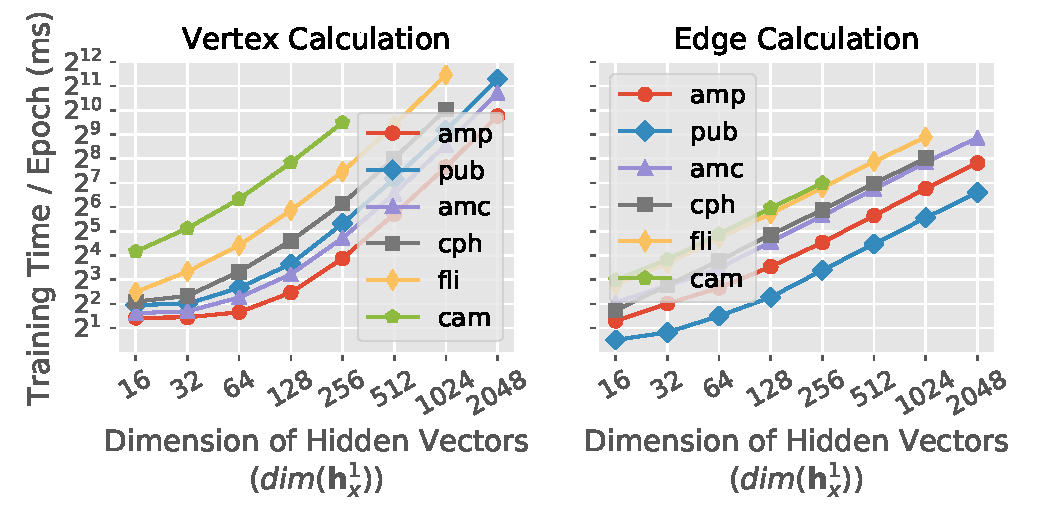
\includegraphics[width=0.7\textwidth]{../figs/experiments/exp_hyperparameter_on_vertex_edge_phase_time_ggnn.pdf}}\\
            \subfloat[Inference]{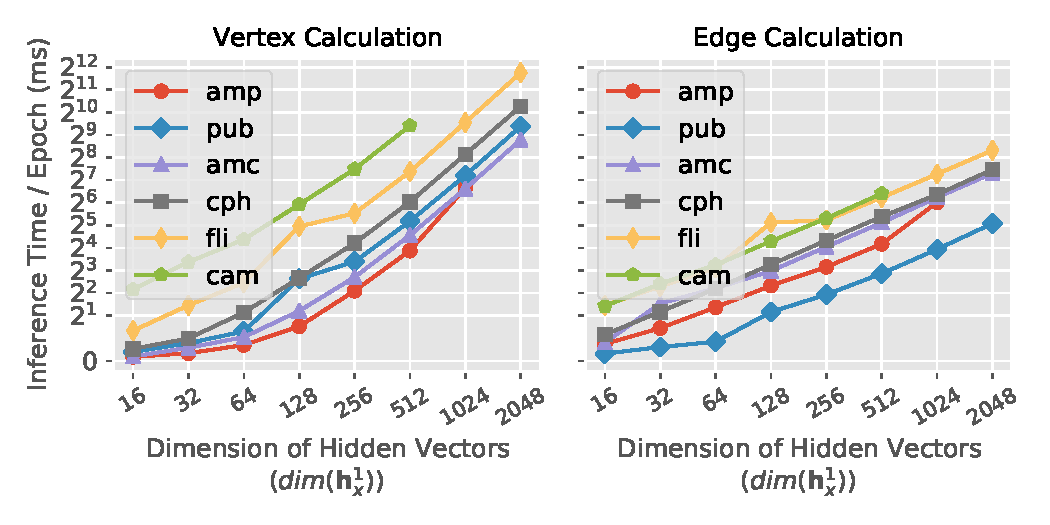
\includegraphics[width=0.7\textwidth]{../figs/experiments/exp_hyperparameter_on_inference_vertex_edge_phase_time_ggnn.pdf}}
            \caption{Effects of hyper-parameters on the vertex/edge calculation time of GGNN.}
            \label{fig:compare_effect_of_hyperparameter_on_time}
    \end{figure}
        
    The effects of hyper-parameters on inference memory usage were also same as training.
    %
    Taking GAT as an example, Figure~\ref{fig:compare_effect_of_hyperparameter_on_memory_usage} in the response (Figure X and Figure X in the revised manuscript) shows the peak memory usage during training and inference under different values of hyper-parameters.
        %
    The trends of the curves in Figure~\ref{fig:compare_effect_of_hyperparameter_on_memory_usage_training} and Figure~\ref{fig:compare_effect_of_hyperparameter_on_memory_usage_inference} were highly similar.
        %
    The memory usage of training and inference \emph{both} grew linearly as the dimension of each head and the number of heads increased.
        %
    We observed similar phenomena in the other GNNs.
        %
    \begin{figure}[H]
            \centering
            \subfloat[Training\label{fig:compare_effect_of_hyperparameter_on_memory_usage_training}]{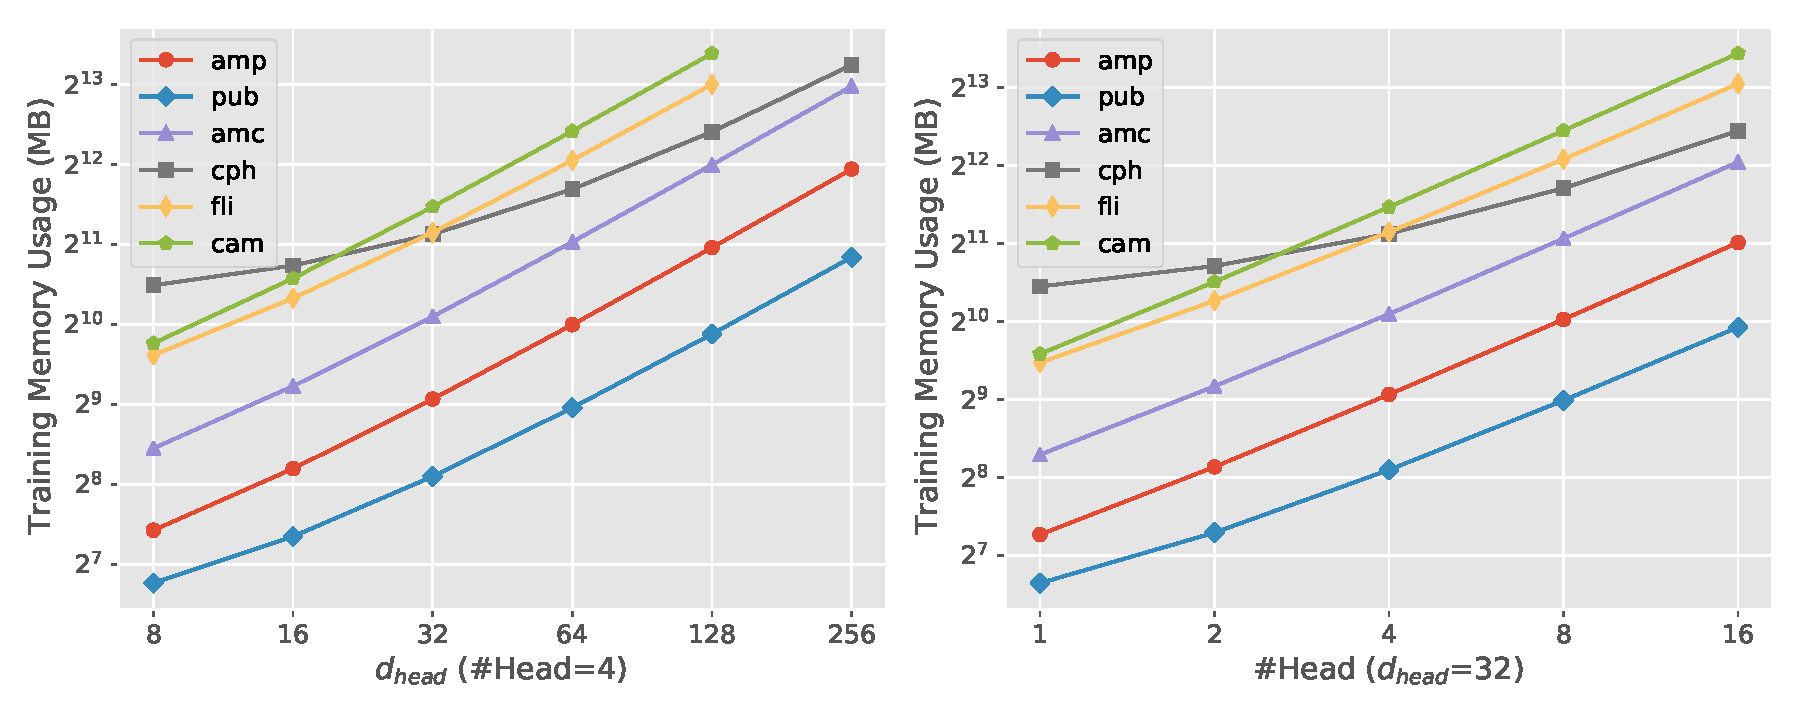
\includegraphics[width=0.6\textwidth]{../figs/experiments/exp_hyperparameter_on_memory_usage_gat.pdf}}\\
            \subfloat[Inference\label{fig:compare_effect_of_hyperparameter_on_memory_usage_inference}]{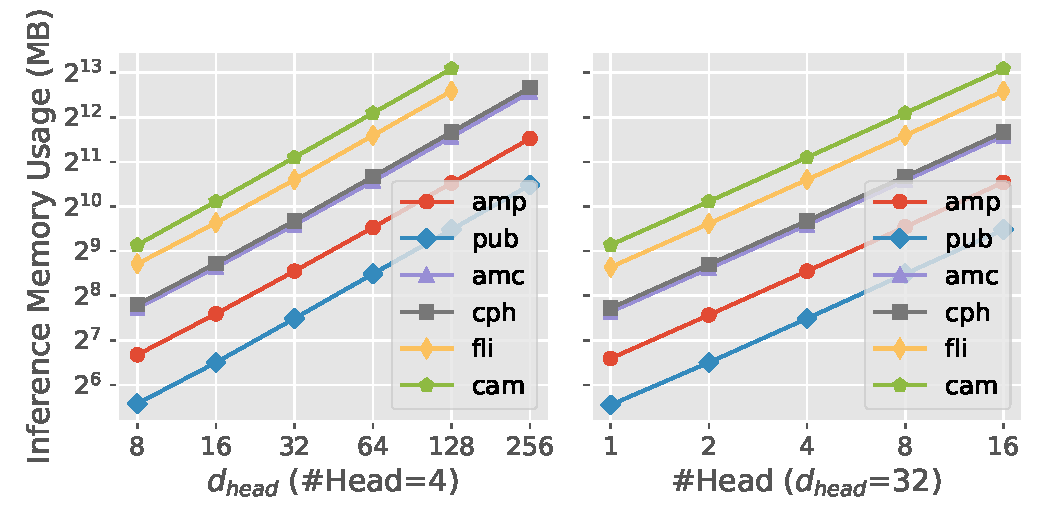
\includegraphics[width=0.6\textwidth]{../figs/experiments/exp_hyperparameter_on_inference_memory_usage_gat.pdf}}
            \caption{Effects of hyper-parameters on peak memory usage of GAT.}
            \label{fig:compare_effect_of_hyperparameter_on_memory_usage}
    \end{figure}
        
    \paragraph{Section 4.2 ``Time Breakdown Analysis''}    
    We have added a new subsection Section 4.2.4 ``Performance Bottlenecks in Inference'' in Section 4.2 to conduct time breakdown analysis for GNN inference and compare the differences between training and inference.

    We found that the performance characteristics of GNN inference were highly similar to training on the \emph{layer} level and the \emph{step} level.
    %
    In this reply, we used GCN as an example.
    %
    We made similar observations in the other GNNs.
    %
    Figure~\ref{fig:compare_layer_level_time_breakdown} in the response compares the time breakdowns of GCN on the layer level of training and inference.
    %
    The time breakdowns were very similar.
    %
    Figure~\ref{fig:compare_effect_of_degree} in the response compares the effects of the average degree on the edge/vertex calculation time during training and inference.
    %
    The curves in the two sub-figures of Figure~\ref{fig:compare_effect_of_degree} have similar trends.
    %
    \emph{The edge calculation stage dominated both the training and inference time}.
    %
    Figure~\ref{fig:compare_time_breakdown_of_edge_calculation} in the response further compares the time breakdowns on the step level of the edge calculation stage.
    %
    The proportion of each step was very similar between training and inference.
    %
    The results indicated that \emph{the performance bottlenecks of training and inference were same on the layer level and step level}.

    
    \begin{figure}[H]
            \subfloat[Training]{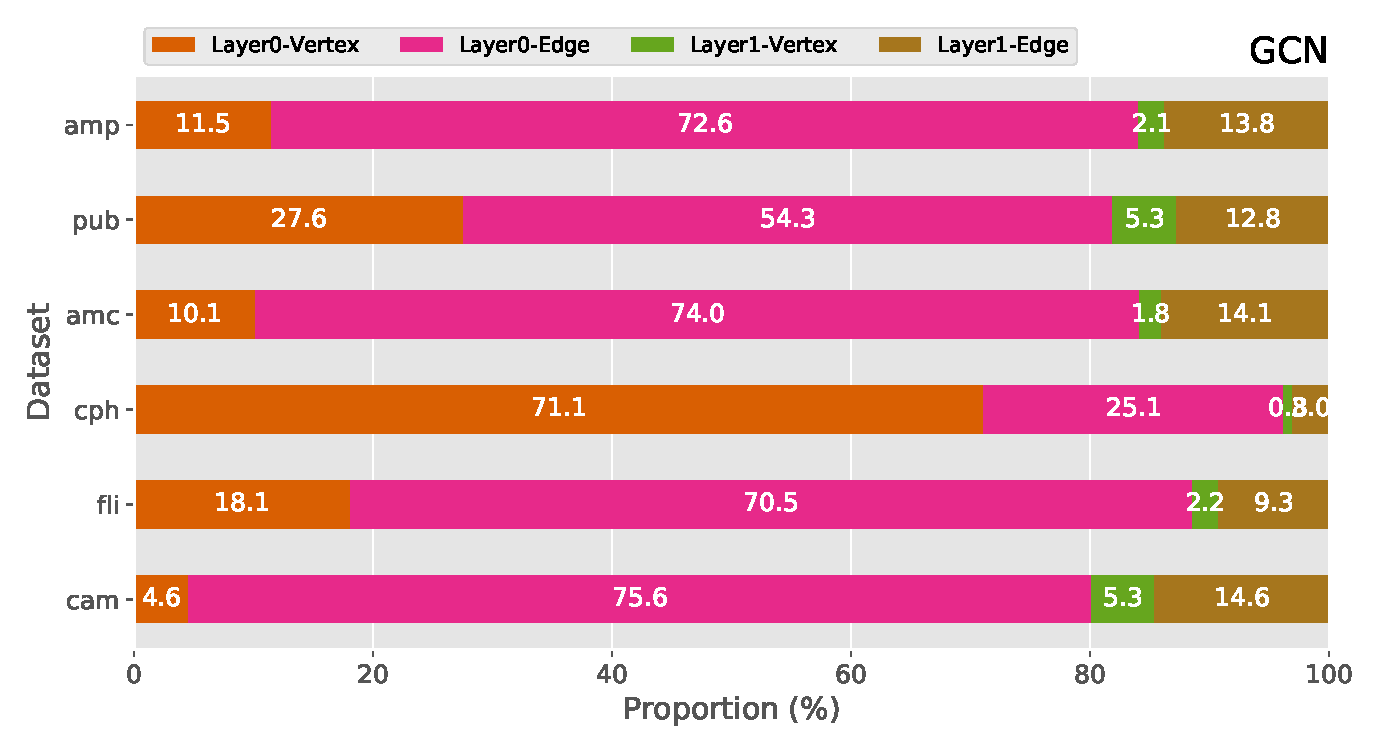
\includegraphics[width=0.5\columnwidth]{../figs/experiments/exp_layer_time_proportion_gcn.pdf}}
            \subfloat[Inference]{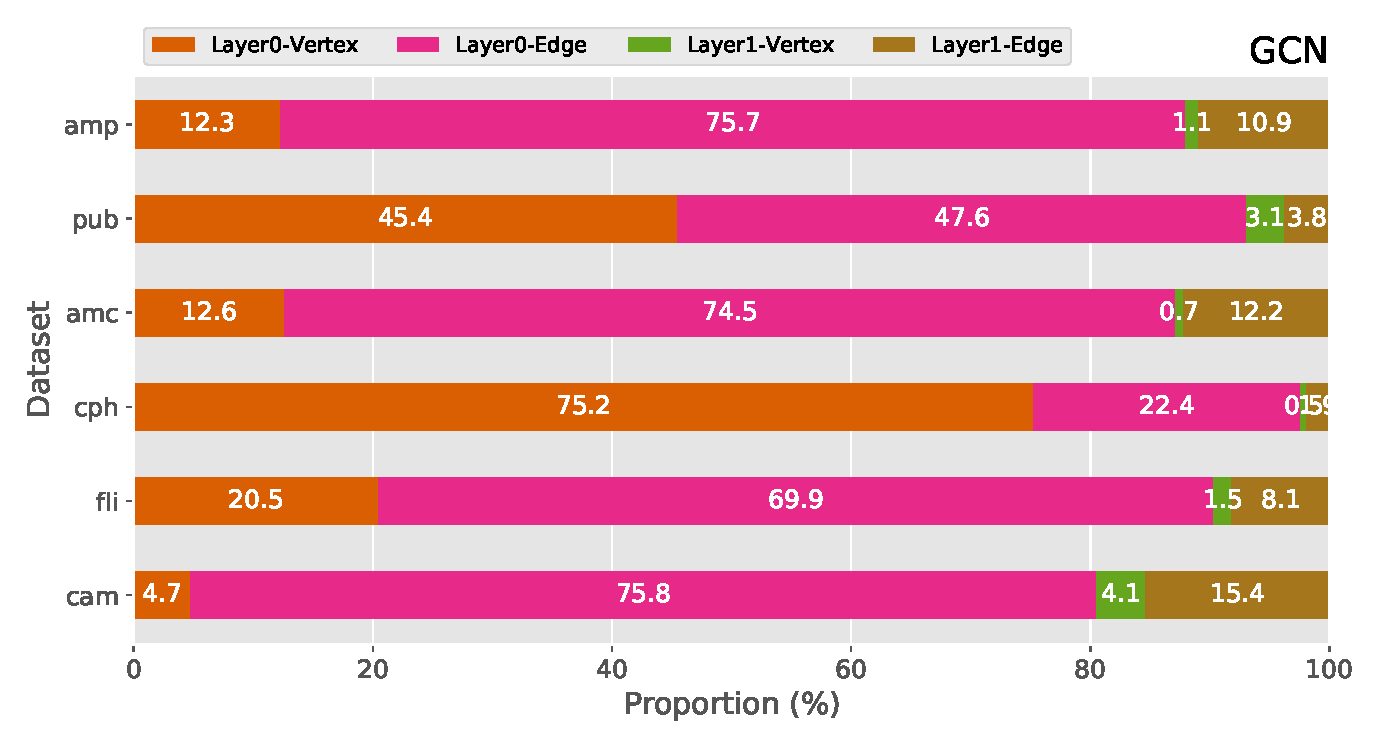
\includegraphics[width=0.5\columnwidth]{../figs/experiments/exp_inference_full_layer_time_proportion_gcn.pdf}}
            \caption{Time breakdowns on the layer level of GCN.}
            \label{fig:compare_layer_level_time_breakdown}
    \end{figure}
    %
    \begin{figure}[H]
                \subfloat[Training\label{fig:compare_effect_of_degree_training}]{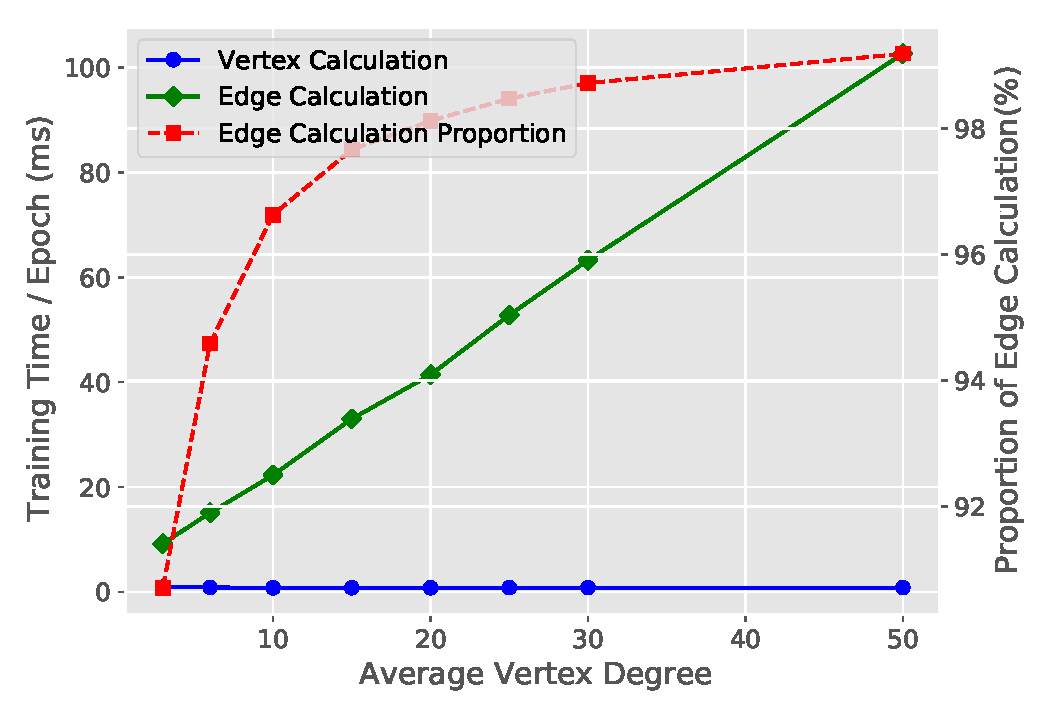
\includegraphics[width=0.5\columnwidth]{../figs/experiments/exp_avg_degree_on_vertex_edge_cal_time_gcn.pdf}}
                \subfloat[Inference\label{fig:compare_effect_of_degree_inference}]{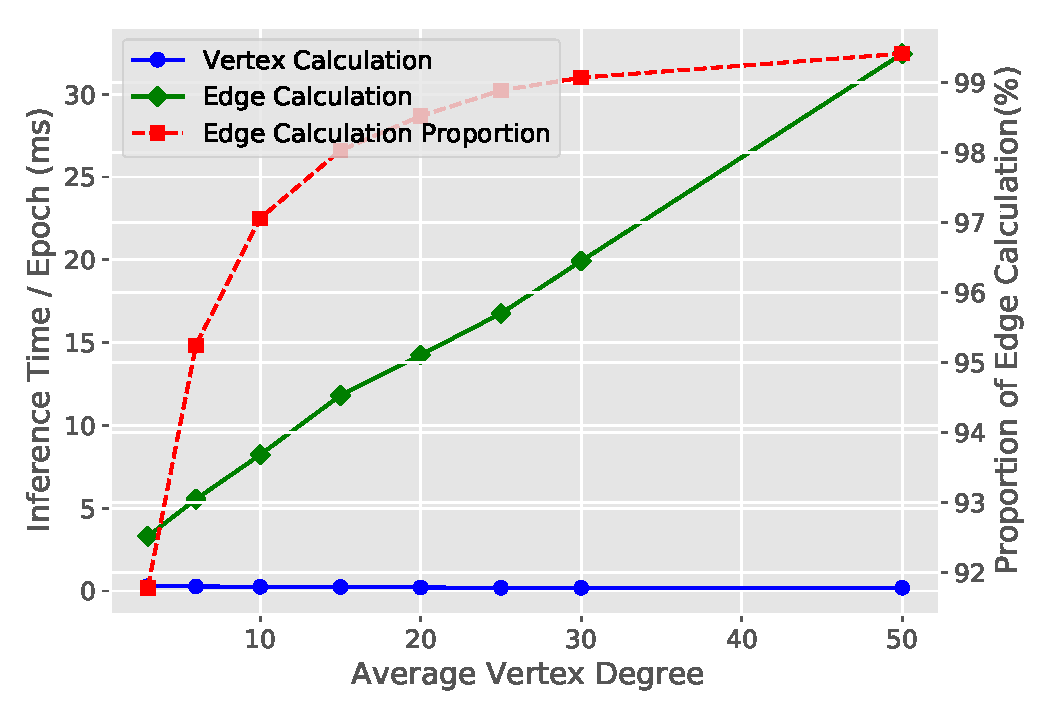
\includegraphics[width=0.5\columnwidth]{../figs/experiments/exp_inference_full_avg_degree_on_vertex_edge_cal_time_gcn.pdf}}
                \caption{Effects of the average degree on the edge/vertex calculation time of GCN. Graphs were generated by fixing the number of vertices as 50,000.}
                \label{fig:compare_effect_of_degree}
    \end{figure}
    %
    \begin{figure}[H]
                \subfloat[Training]{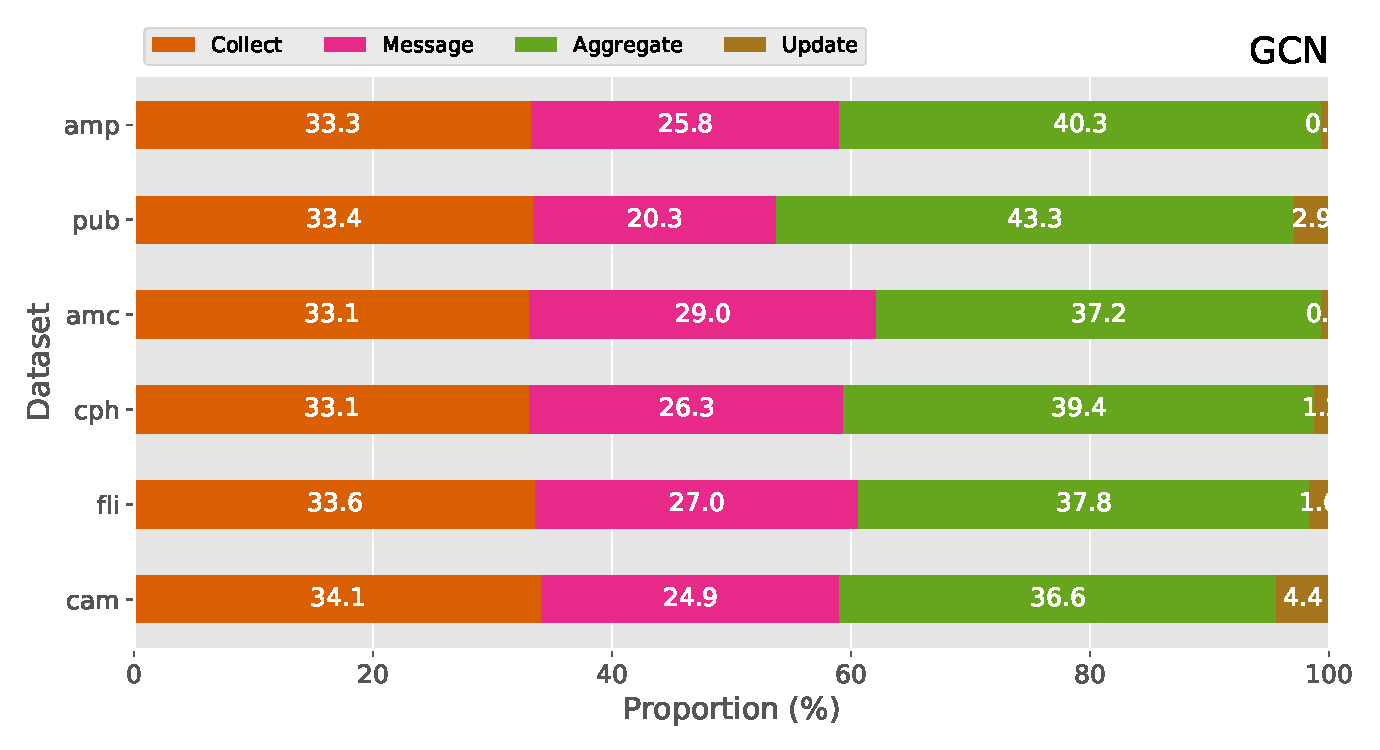
\includegraphics[width=0.5\columnwidth]{../figs/experiments/exp_edge_calc_decomposition_gcn.pdf}}
                \subfloat[Inference]{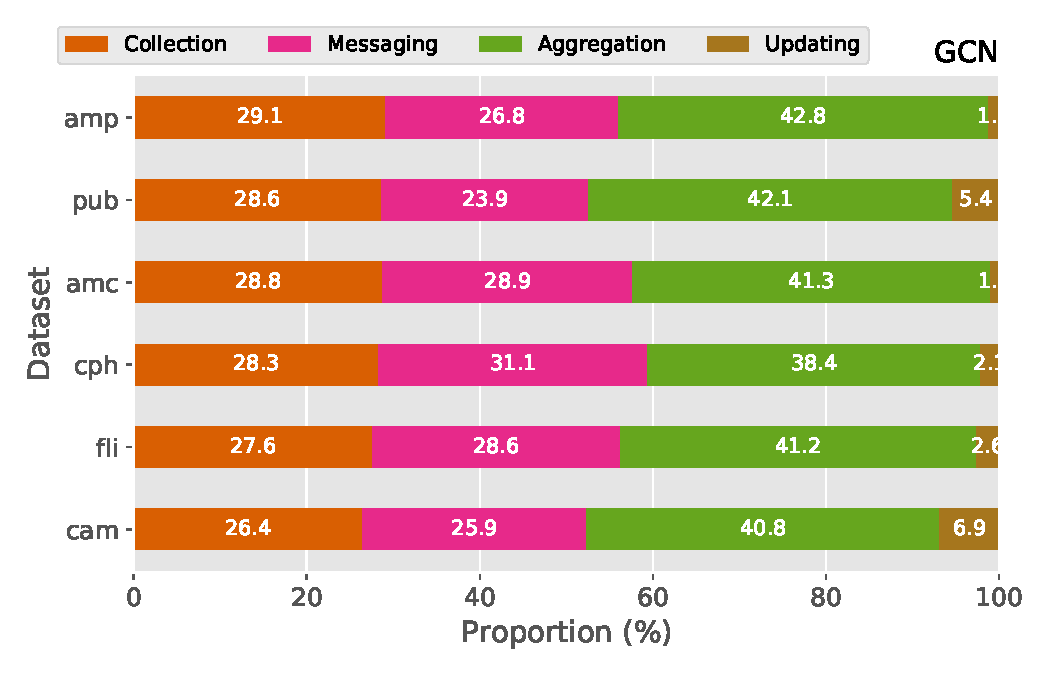
\includegraphics[width=0.5\columnwidth]{../figs/experiments/exp_inference_full_edge_calc_decomposition_gcn.pdf}}
                \caption{Time breakdowns on the step level of the edge calculation stage of GCN.}
                \label{fig:compare_time_breakdown_of_edge_calculation}
    \end{figure}
    
    The main differences between training and inference were reflected in two aspects: the wall-clock time and the top time-consuming basic operators.
    
    The inference time was much less than the training time.
    %
    Figure~\ref{fig:compare_wall_clock_time_of_training_and_inference} in the response (Figure X in the revised manuscript) compares the wall-clock time of training and inference on the \texttt{amp}, \texttt{amc}, and \texttt{fli} datasets.
    %
    The results on the other datasets were similar.
    %
    Since the inference only conducted the forward propagation from the input layer to the prediction layer, the time of inference was very close to the time of the forward phase in training.
    %
    The inference time was 34\% (GCN), 32\% (GGNN), 25\% (GAT), and 32\% (GaAN) of the training time, averaged over all datasets.
    
    \begin{figure}[H]
        \centering
        \subfloat[\texttt{amc}]{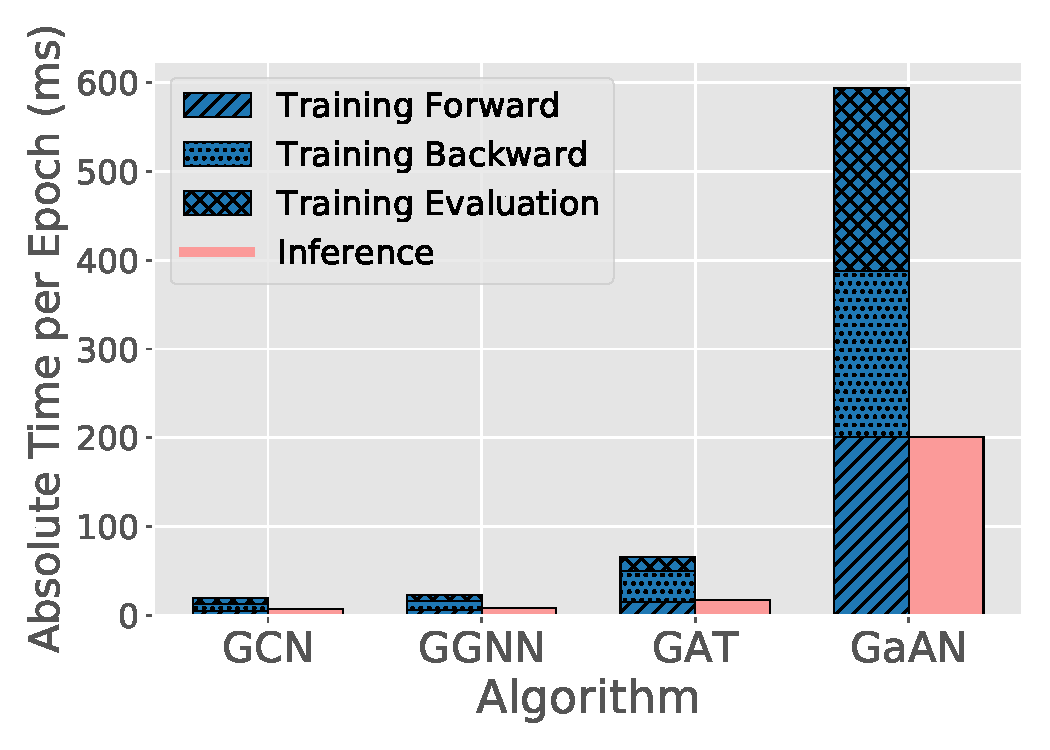
\includegraphics[width=0.3\columnwidth]{../figs/experiments/exp_time_comparison_between_training_inference_amazon-computers.pdf}}
        \subfloat[\texttt{amp}]{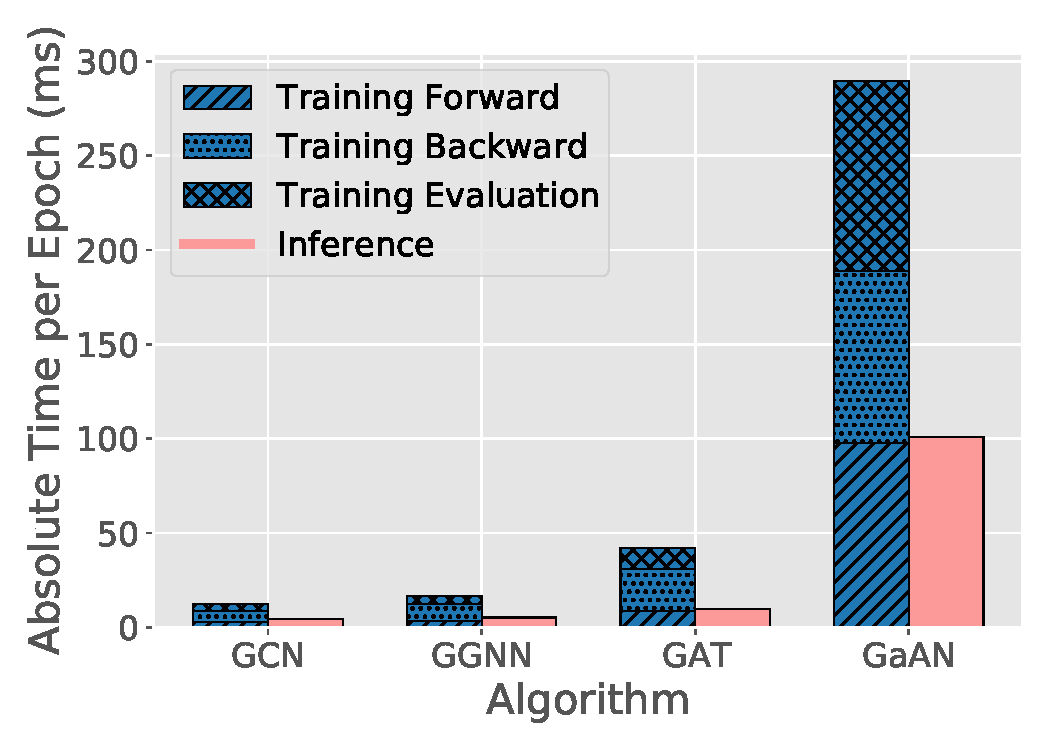
\includegraphics[width=0.3\columnwidth]{../figs/experiments/exp_time_comparison_between_training_inference_amazon-photo.pdf}}
        \subfloat[\texttt{fli}]{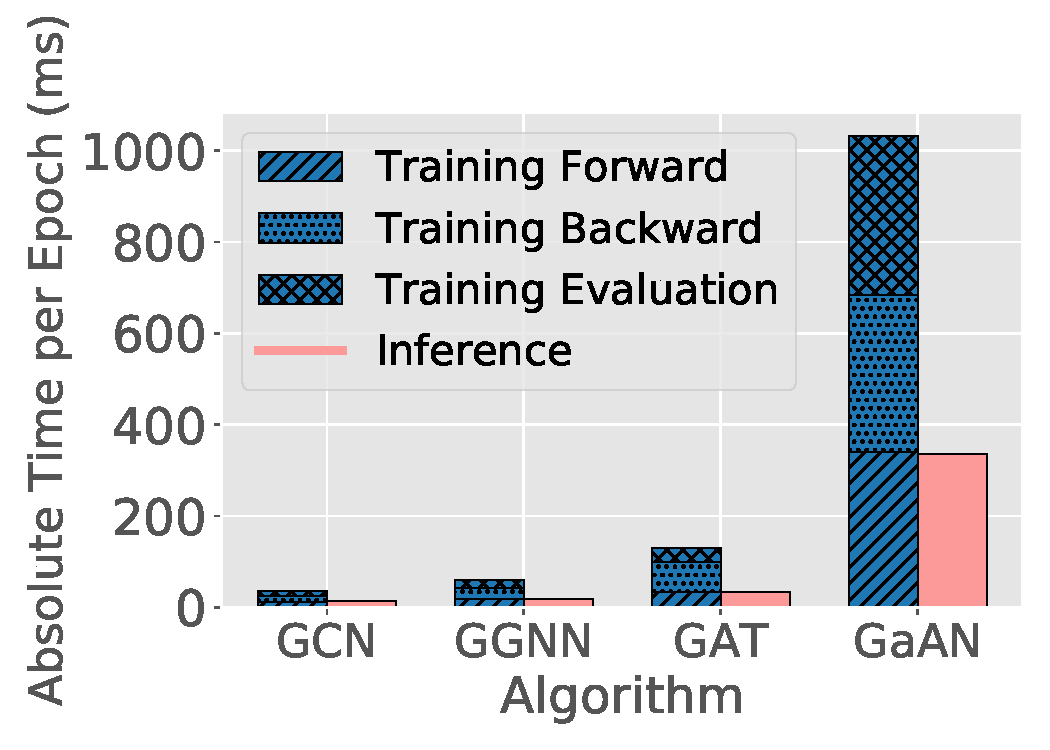
\includegraphics[width=0.3\columnwidth]{../figs/experiments/exp_time_comparison_between_training_inference_flickr.pdf}}
        \caption{Wall-clock training/inference time on different datasets.}
        \label{fig:compare_wall_clock_time_of_training_and_inference}
    \end{figure}
    
    The top time-consuming basic operators of training and inference also showed a certain degree of difference.
    %
    Some of the top time-consuming operators during training were replaced by new operators in inference.
    %
    Figure~\ref{fig:compare_top_time_consuming_basic_operators} in the response (Figure X in the revised manuscript) compares the top 5 time-consuming basic operators in training and inference.
    %
    For GCN, the \texttt{index} operator used in the prediction layer became the new top 5 time-consuming operator, replacing the \texttt{gather} operator used in the backward phase in training.
    %
%    The basic operators related to the edge calculation (\texttt{scatter\_add}, \texttt{index\_select}, and \texttt{mul}) still consumed the majority of the inference time.
    %
    For GGNN, \texttt{index} operator in the prediction layer also became one of the top 5 time-consuming basic operators.
    %
%    Due to the high time complexity of the vertex updating function $\gamma$ in GGNN, the basic operators related to the vertex calculation stage (\texttt{mm} and \texttt{thnn\_fused\_gru\_cell}) still consumed near half of the inference time.
    %
    For GAT, the \texttt{input\_put\_impl} operator (used in the backward phase) in Figure~\ref{fig:compare_top_time_consuming_basic_operators}e was replaced by the \texttt{scatter\_add} operator used in the forward edge calculation in Figure~\ref{fig:compare_top_time_consuming_basic_operators}f.
    %
%    The \texttt{scatter\_add} operator was related to the edge calculation step.
    %
    For GaAN, the \texttt{mm} operator was replaced by the \texttt{cat} operator used in the vertex updating function.
    
    Although some specific time-consuming operators were different, the performance bottlenecks on the operator level were same for training and inference.
    %
    The matrix multiplication \texttt{mm} and the element-wise multiplication \texttt{mul} operators were still time-consuming for inference, making GNN inference also {suitable for GPUs}.
    %
    The basic operators related to the collection and aggregation steps in the edge calculation still consumed non-trivial time in inference.
    
    \begin{figure}[H]
        \centering
        \subfloat[GCN, Training]{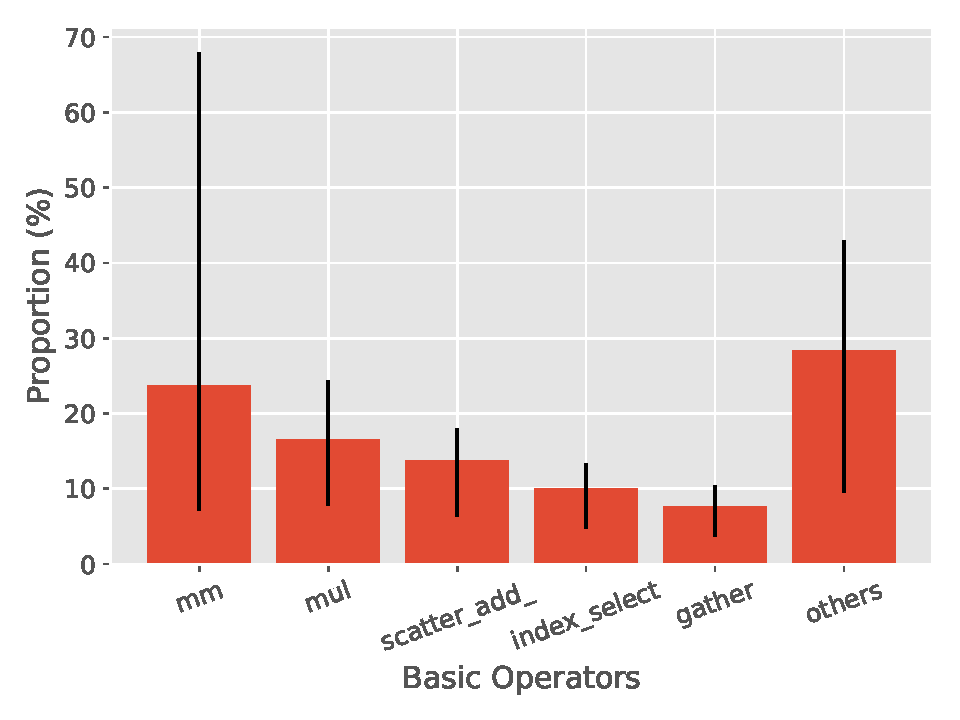
\includegraphics[width=0.35\columnwidth]{../figs/experiments/exp_top_basic_ops_gcn.pdf}}
         \subfloat[GCN, Inference]{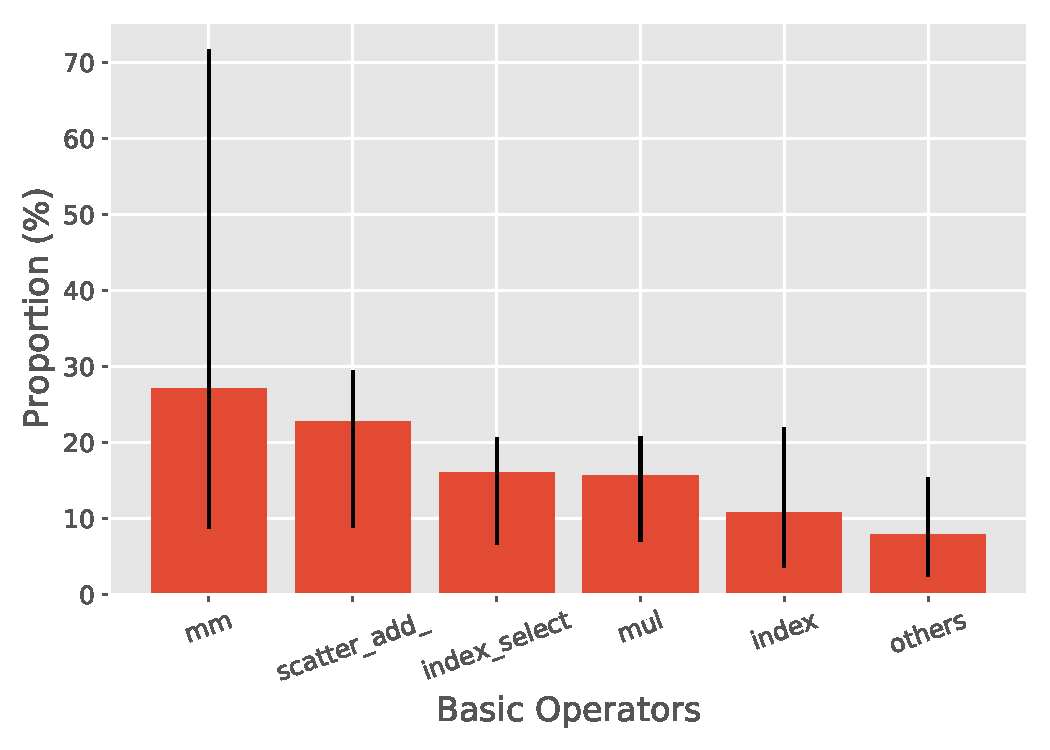
\includegraphics[width=0.35\columnwidth]{../figs/experiments/exp_inference_full_top_basic_ops_gcn.pdf}}\\
        \subfloat[GGNN, Training]{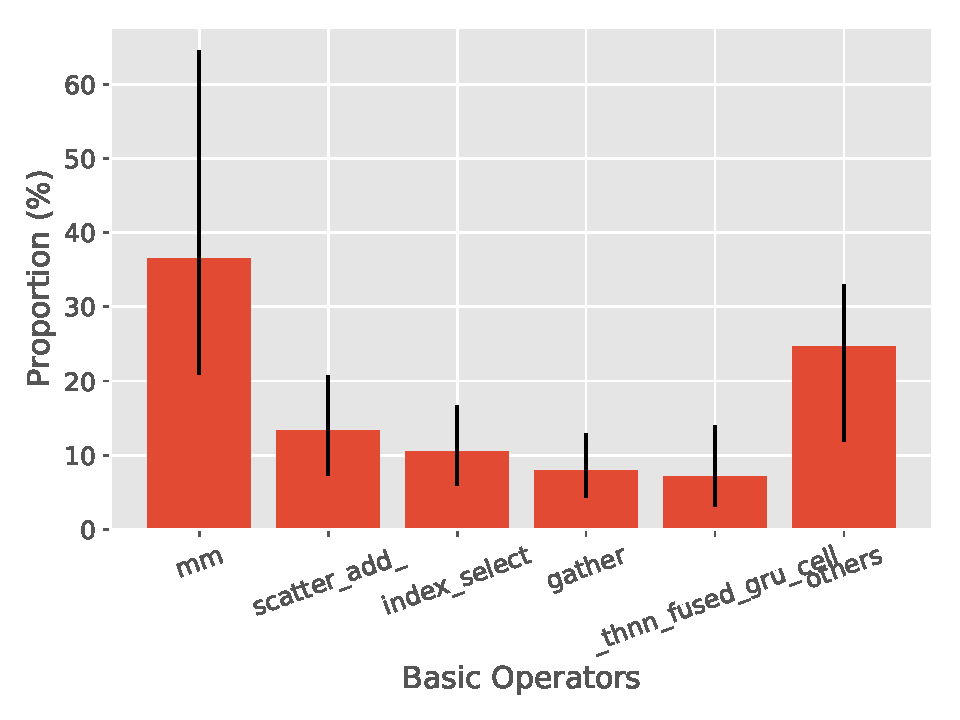
\includegraphics[width=0.35\columnwidth]{../figs/experiments/exp_top_basic_ops_ggnn.pdf}}
         \subfloat[GGNN, Inference]{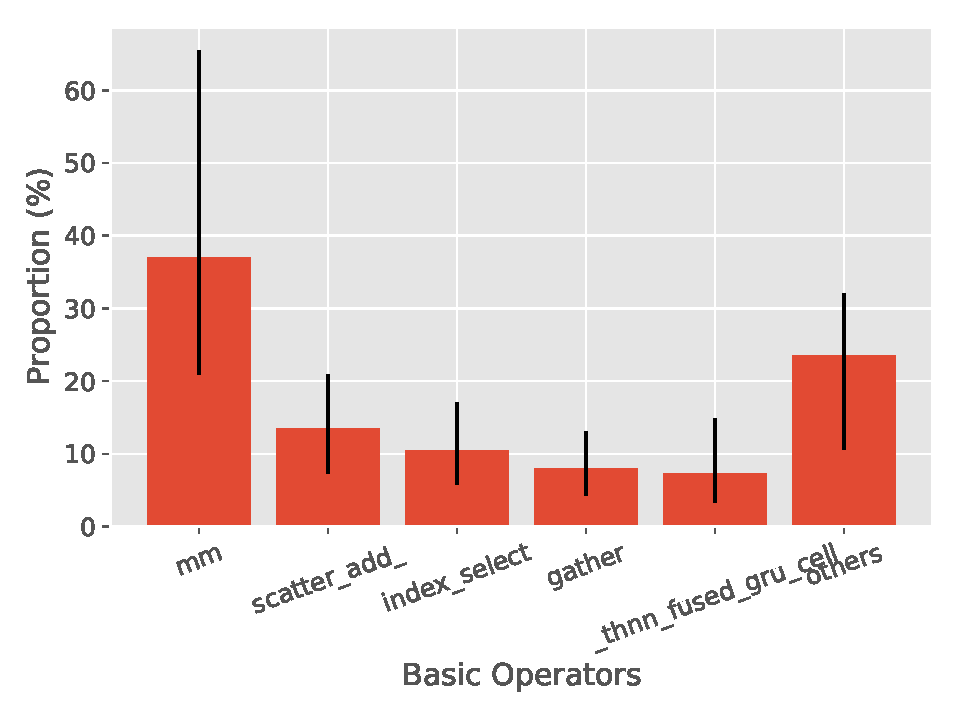
\includegraphics[width=0.35\columnwidth]{../figs/experiments/exp_inference_full_top_basic_ops_ggnn.pdf}}\\
        \subfloat[GAT, Training]{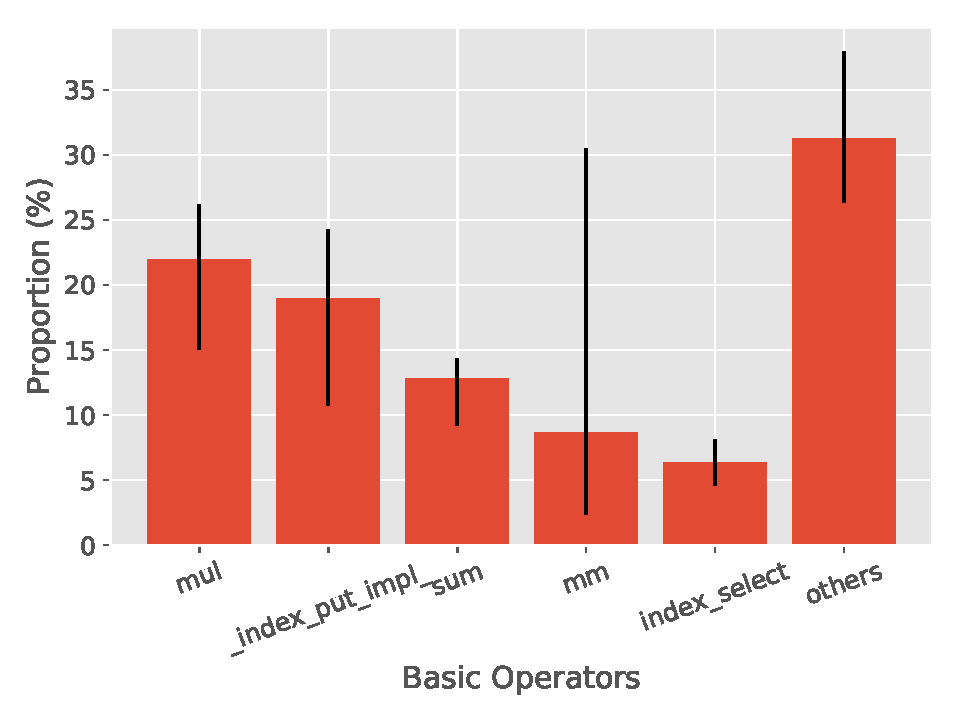
\includegraphics[width=0.35\columnwidth]{../figs/experiments/exp_top_basic_ops_gat.pdf}}
         \subfloat[GAT, Inference]{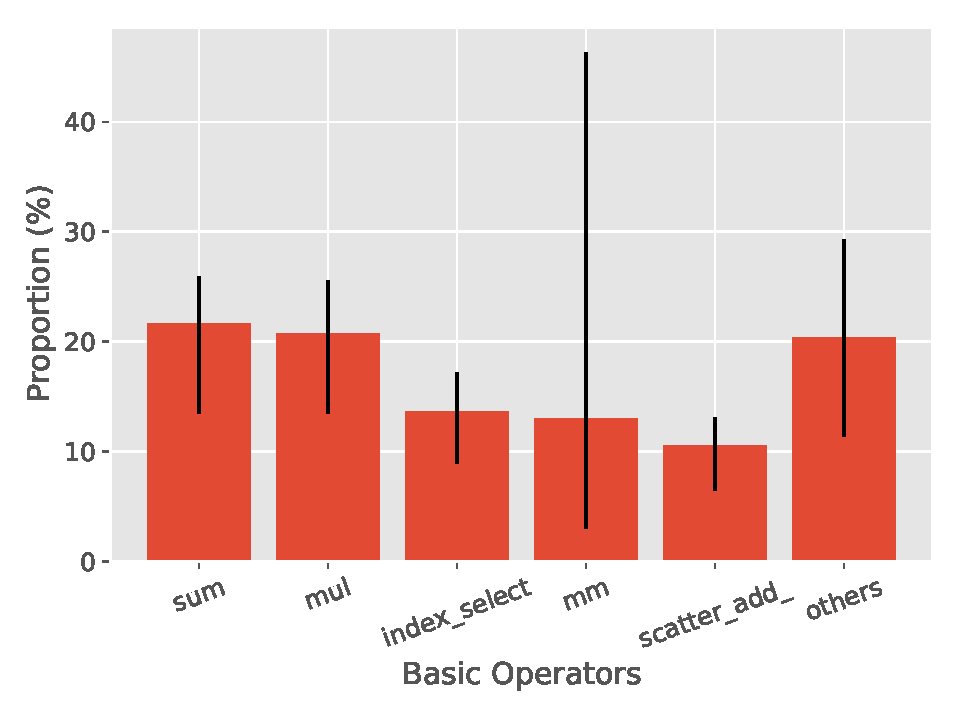
\includegraphics[width=0.35\columnwidth]{../figs/experiments/exp_inference_full_top_basic_ops_gat.pdf}}\\
        \subfloat[GaAN, Training]{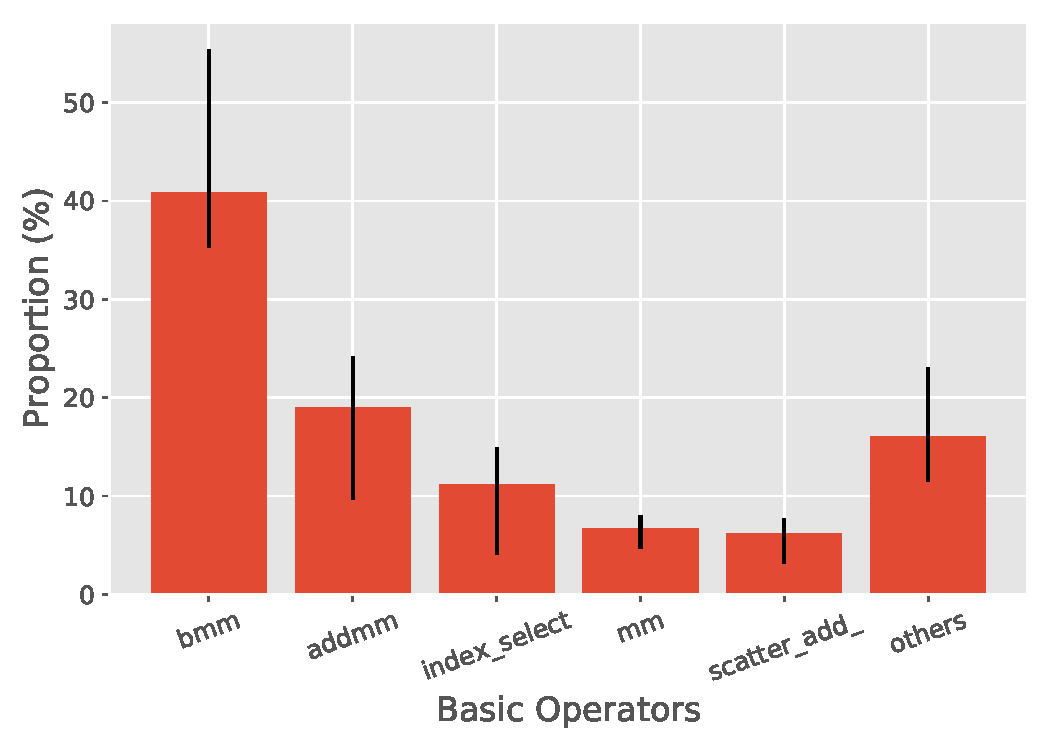
\includegraphics[width=0.35\columnwidth]{../figs/experiments/exp_top_basic_ops_gaan.pdf}}
         \subfloat[GaAN, Inference]{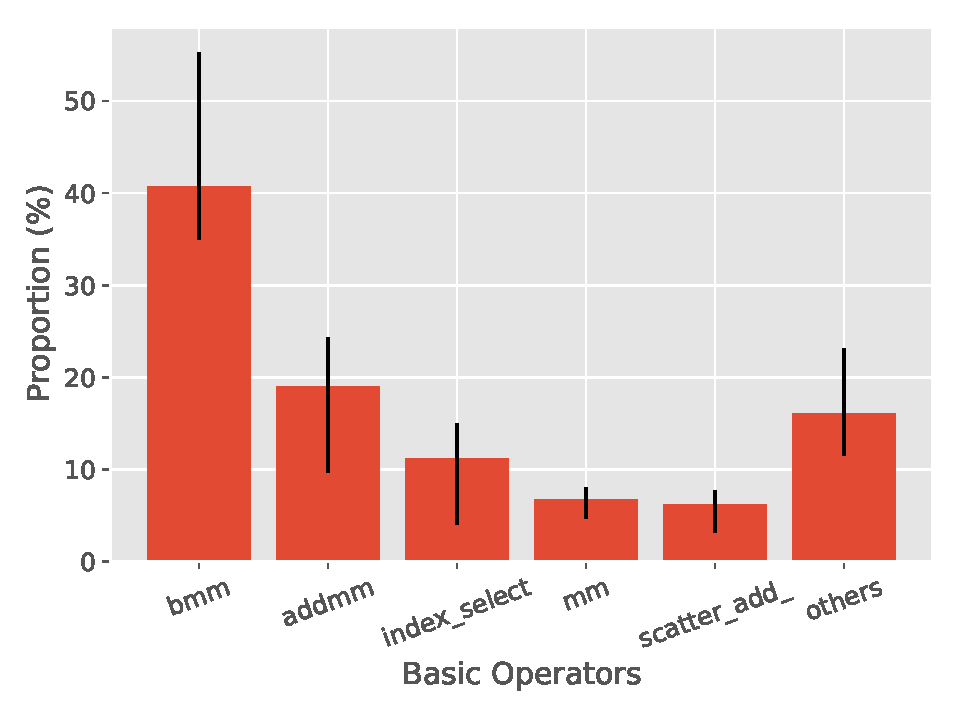
\includegraphics[width=0.35\columnwidth]{../figs/experiments/exp_inference_full_top_basic_ops_gaan.pdf}}\\
         
         \caption{Top 5 time-consuming basic operators of typical GNNs. The time proportion of each basic operator was averaged over all datasets with the error bar indicating the maximum and the minimum.}
         \label{fig:compare_top_time_consuming_basic_operators}
         
    \end{figure}
    
    \paragraph{Section 4.3 ``Memory Usage Analysis''}
         
     In the end of Section 4.3, we added a new paragraph ``Memory Usage of Inference'' to compare the memory usage of inference and training.
     %
     
     %
     Figure~\ref{fig:compare_memory_expasion_ratio} in the response (Figure X in the revised manuscript) compares the memory expansion ratios of typical GNNs during training and inference.
     %
     Since no intermediate results had to be cached during inference of GGNN, GAT, and GaAN, the memory expansion ratios of inference were much less than training for the three GNNs.
     %
     The MERs of inference were 45\% to 83\% (GGNN), 52\% to 61\% (GAT), and 37\% to 69\% (GaAN) of training.
     %
     However, the MERs were still high, disallowing inferencing with big graphs.
     %
     To handle big graphs, sample-based inference was necessary.
     
     \begin{figure}[H]
        \subfloat[Training]{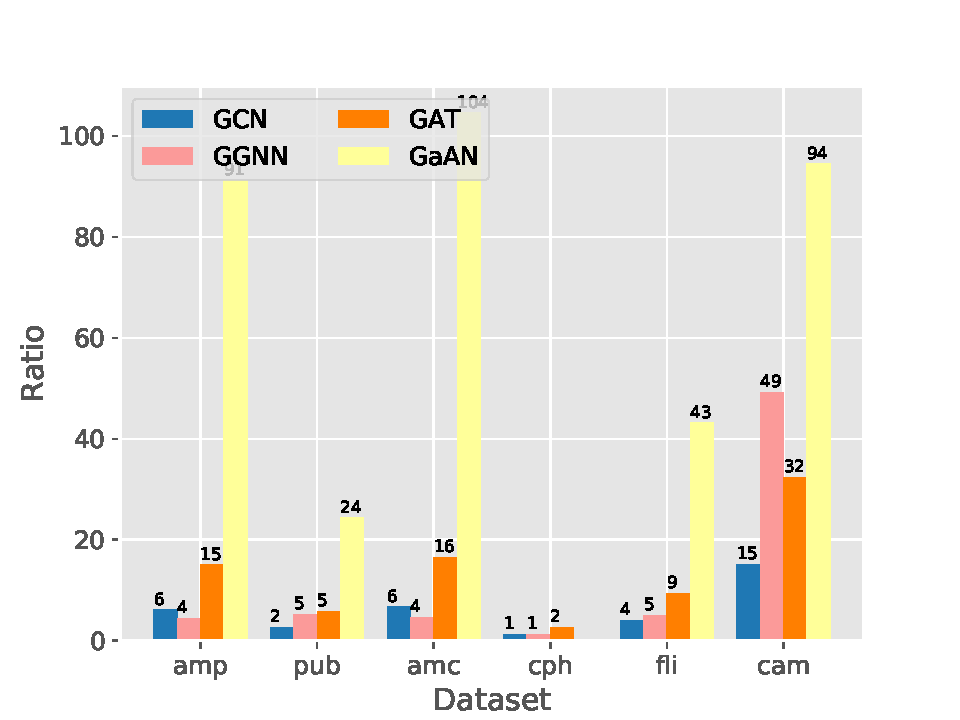
\includegraphics[width=0.5\columnwidth]{../figs/experiments/exp_memory_expansion_ratio.pdf}}
        \subfloat[Inference]{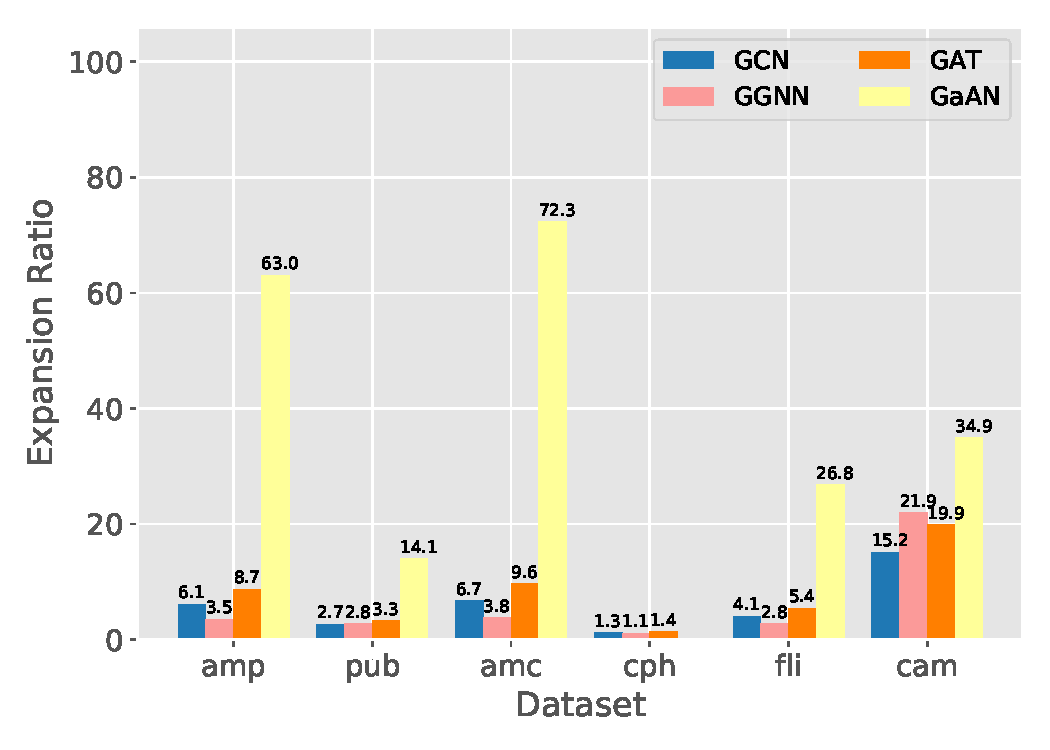
\includegraphics[width=0.5\columnwidth]{../figs/experiments/exp_inference_full_memory_expansion_ratio.pdf}}
        \caption{Memory expansion ratios of typical GNNs.}
        \label{fig:compare_memory_expasion_ratio}
     \end{figure}
     
     \paragraph{Section 4.4 ``Effects of Sampling Techniques on Performance''}
     %
     In Section 4.4, we added a new subsection  Section 4.4.4 ``Performance Bottlenecks in Inference'' to discuss the performance bottlenecks in sample-based inference.
     
     Sample-based inference was an effective technique to handle big graphs.
     %
     Taking the node classification task as an example, to predict labels for a given set of vertices $\mathcal{V}_{predict}$, the inference sampler sampled a subgraph containing complete $L$-hop neighborhoods of all vertices in $\mathcal{V}_{predict}$, where $L$ was the number of GNN layers.
     %
     Since the real-world graphs often had small-world property, the size of the sampled subgraph increased quickly as the number of vertices in $\mathcal{V}_{predict}$ (i.e., batch size) increased.
     %
     Figure~\ref{fig:sampled_graph_size} (Figure X in the revised manuscript) shows how the relative batch size ($\frac{|\mathcal{V}_{predict}|}{|\mathcal{V}|}$) affected the average degree and the number of edges of the sampled subgraphs during inference.
     %
     When the relative batch size was 10\%, the number of edges in the sampled subgraphs were close to the number of edges in the whole graph in most datasets.
     %
     In order to limit the memory usage during inference, the batch size used should be very small.
     
     \begin{figure}[H]
        \centering
        \subfloat[Average degree]{    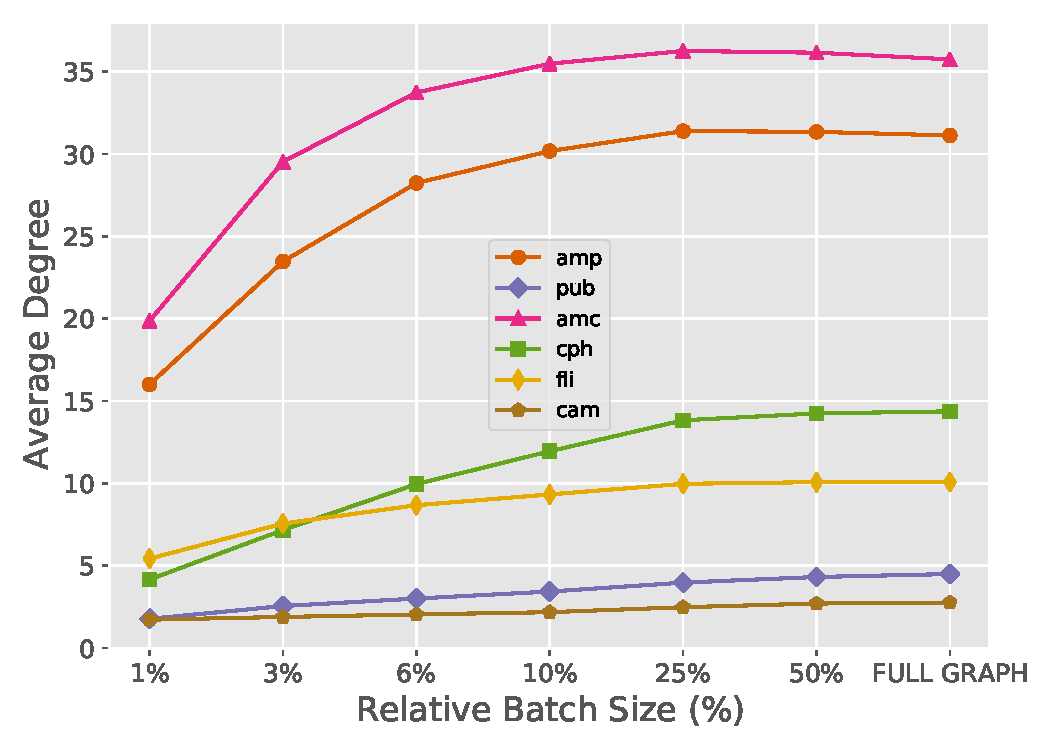
\includegraphics[width=0.5\columnwidth]{../figs/experiments/exp_inference_sampling_graph_info_inference_sampler_avg_degrees.pdf}}
        \subfloat[Number of edges]{    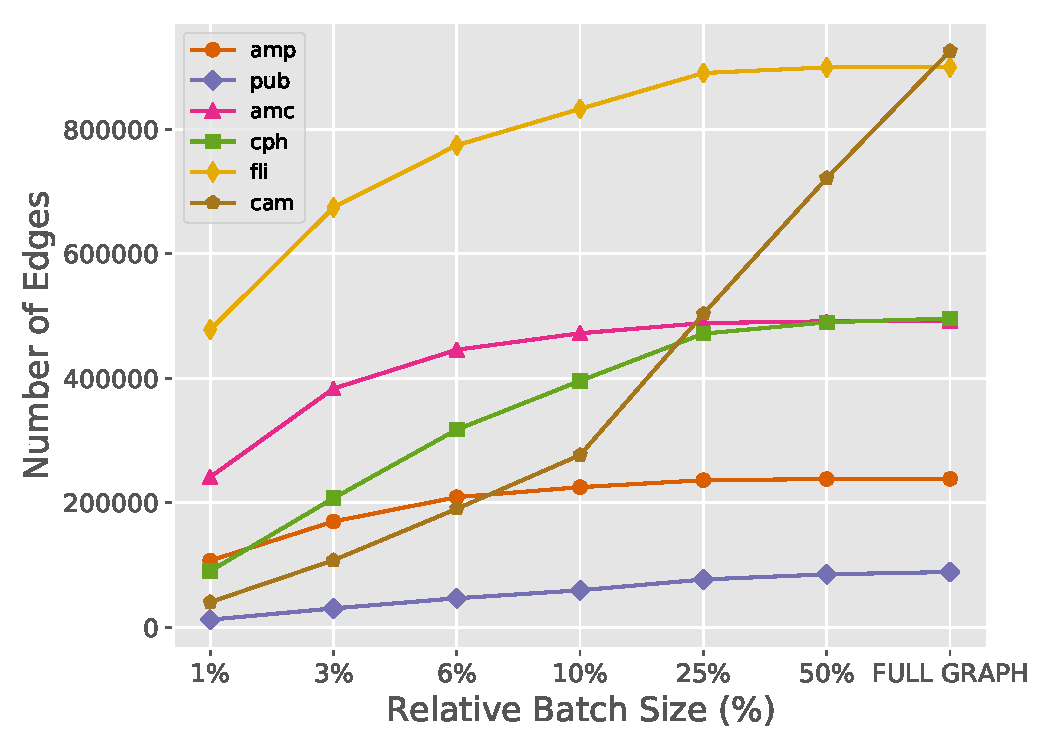
\includegraphics[width=0.5\columnwidth]{../figs/experiments/exp_inference_sampling_graph_info_inference_sampler_edges.pdf}}
        
        \caption{Characteristics of the sampled subgraphs produced by the inference sampler under different relative batch sizes.}
        \label{fig:sampled_graph_size}
     \end{figure}
     
     However, the overheads brought by sampling and data transfering from CPU to GPU became obvious when the batch size was small.
     %
     Figure~\ref{fig:time_breakdown_of_inference_sampler} (Figure X in the revised manuscript) shows the time breakdowns of sample-based inference on different datasets.
     %
     On the \texttt{amp} and \texttt{cam} datasets, the sampling time even accounted for near half of the total inference time.
     %
     The results indicated that the current implementation of inference sampler in PyG was also inefficient.
     %
     Improving its efficiency could significantly reduce the inference time.
     
     
     \begin{figure}[H]
        \centering
        \subfloat[Batch Size = 1024]{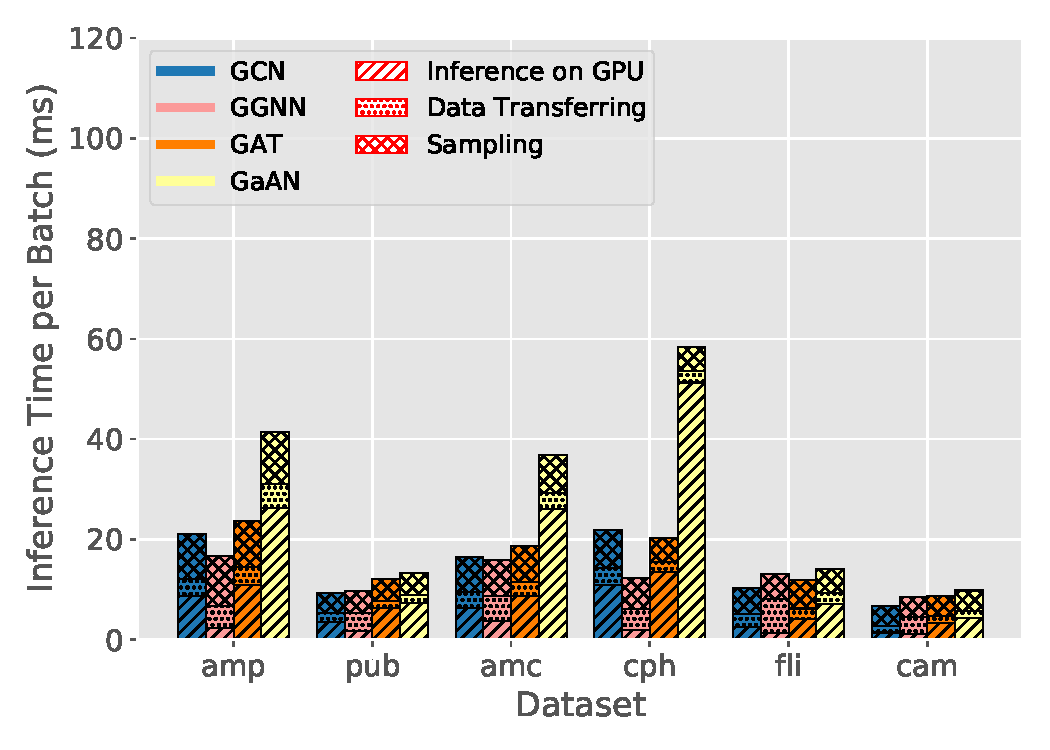
\includegraphics[width=0.5\columnwidth]{../figs/experiments/exp_inference_sampling_fix_batch_size_train_time_stack_1024.pdf}}
        \subfloat[Batch Size = 2048]{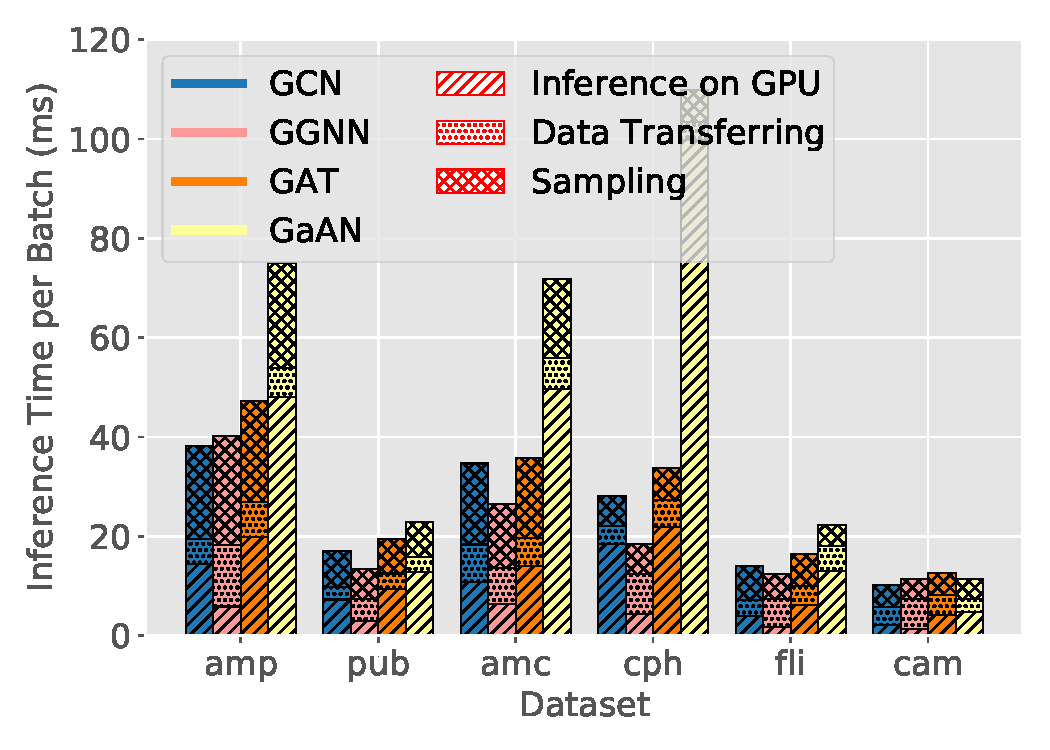
\includegraphics[width=0.5\columnwidth]{../figs/experiments/exp_inference_sampling_fix_batch_size_train_time_stack_2048.pdf}}
        \caption{Inference time per batch breakdown under different batch sizes.}
        \label{fig:time_breakdown_of_inference_sampler}
     \end{figure}
\end{reply}

% Begin a new reviewer section
\reviewersection

\begin{point}
    In the paper, authors accomplished a unique study and analysis on GNN models training complexity.  The articles first review and development history of GNNs and creatively model all architectures as input layers, intermediate layers of graph neurons and prediction layers. And they quantitatively summarize the time and space complexity of 4 representative GNNs, including graph convolution, gated recurrent graph net, graph attention net and GraphSage. Most importantly, the article first break down complexity into operator level and offered analysis of good granularity, giving reader more guidance in future study. At last, the solid experiments included the study of effects of hyper-parameters and a comparison of two major sampling techniques: neighbor sampling and cluster sampling.
\end{point}

\begin{reply}
    Thank you for your positive comments on our manuscript.
    %
    We have carefully revised the manuscript according to your kindly comments and suggestions in the following points.
    %
    We highlight our modifications with red squares point by point in the annotated version of the revised manuscript.
\end{reply}

\begin{point}
    In general, the paper was well written and organized with good structure and clear narratives. Just some minor language errors like line Page 8, Line 208, "In active graph neurons" =\textgreater "Inactive graph neurons".
\end{point}

% R2Q1
\begin{reply}
    We feel really sorry for our carelessness.
    %
    We have proofread our revised manuscript to eliminate such language errors as much as we can.
\end{reply}

% R2Q2
\begin{point}
    I was impressed by the way that authors categorize layers and operators in GNNs, very clear and instructive.
    
    It is also pretty neat to divide layer time complexity into two buckets: vertex calculation and edge calculation. The data model pretty well summarizes mainstream GNN layer architectures. And this analysis is very insightful for layer profiling.
    
    And the experimental evaluation were done over 6 large graph-structured datasets.
\end{point}

\begin{reply}
    Thank you very much for your appreciation.	
\end{reply}

% R2Q3
\begin{point}
    While, one major drawback is that I did not clearly see the analysis complexity v.s. accuracy. For example, in Figure 19 and 20, I did not see network accuracy from those 4 GNNs. There is always tradeoff between model complexity and model performance, and in some scenarios where high complexity is allowed, a sophisticated model of more powerful representation capability is still needed.
\end{point}

\begin{reply}
    Thanks very much for your valuable suggestions.
    %
    The model complexity directly affects both the accuracy and the training time.
    %
    In order to analyze the relationship between model complexity and accuracy, we have conducted two kinds of extra experiments in the revised manuscript: (1) how the hyper-parameters of the GNNs (like the dimension of hidden vectors and the number of heads) affect the accuracy of GNNs (in Section 4.1); (2) how the batch size in the sampling methods affects the accuracy of GNNs (in Section 4.4).
    
    We have added more dataset description related to accuracy evaluation in Section 3.1 ``Experimental Setting''.
    %
    Newly added sentences are marked with underlines in the following quotation.
    
    \begin{myquote}{Section 3.1 ``Experimental Setting''}
    \emph{Datasets}.
    %
    We used six real-world graph datasets as listed in \tablename~\ref{tab:dataset_overview} (in the reply) that were popular in the GNN evaluation [28,31,34,36].
    %
    For directed graphs, PyG converts them into undirected ones during data loading.
    %
    Thus, the average degree of a directed graph $\bar{d}=\frac{2|\mathcal{E}|}{|\mathcal{V}|}$.
    %
    For an undirected graph, the average degree is defined as $\bar{d}=\frac{|\mathcal{E}|}{|\mathcal{V}|}$.
    %
    \ul{For the \texttt{cam} dataset, its vertices were not associated with feature vectors}.
    %
    \ul{Thus, we generated random dense feature vectors for it and excluded it from accuracy evaluation}.
    %
    \ul{For \texttt{amp}, \texttt{amc}, \texttt{cph}, and \texttt{cam}, we used 70\%/15\%/15\% of the vertices as the training/evaluation/test set, respectively}.
    %
    \ul{For \texttt{pub}, we used 500/1000 vertices as the evaluation/test set and the remained as the training set according to [28]}.
    %
    \ul{For \texttt{fli}, we used 50\%/25\%/25\% of the samples as the training/evaluation/test set according to [31]}.
    %
    We also used random graphs generated by the R-MAT graph generator [35] in some experiments, to explore the effects of graph topological characteristics (like average degrees) on performance bottlenecks.
    %
    Input feature vectors of random graphs were random dense vectors with the dimension of 32.
    %
    Vertices of random graphs were classified into 10 classes randomly.
    
    \begin{table}[H]
        \centering
        \begin{tabular}{cccccccc}
            \toprule
            Dataset                                                 & $|\mathcal{V}|$ & $|\mathcal{E}|$ & $\bar{d}$ & $dim(\boldsymbol{v})$ & \#Class & Directed \\
            \midrule
            pubmed (\texttt{pub}) [28]  & 19,717          & 44,324          & 4.5       & 500                   & 3       & Yes      \\
            amazon-photo (\texttt{amp}) [34]     & 7,650           & 119,081         & 31.1      & 745                   & 8       & Yes      \\
            amazon-computers (\texttt{amc}) [34] & 13,752          & 245,861         & 35.8      & 767                   & 10      & Yes      \\
            coauthor-physics (\texttt{cph}) [34] & 34,493          & 247,962         & 14.4      & 8415                  & 5       & Yes      \\
            flickr (\texttt{fli}) [31]                 & 89,250          & 899,756         & 10.1      & 500                   & 7       & No       \\
            com-amazon (\texttt{cam}) [36]               & 334,863         & 925,872         & 2.8       & 32                    & 10      & No       \\
            \bottomrule
        \end{tabular}
        \caption{Dataset overview. $\bar{d}$ represents the average vertex degree. $dim(\boldsymbol{v})$ is the dimension of the input feature vector.}
        \label{tab:dataset_overview}
    \end{table}

    \end{myquote}

    In this reply, we focus on the experiments related to hyper-parameters in Section 4.1.
    %
    We introduce the experimental results of the sampling techniques in Section 4.4 in the next reply.

    Hyper-parameters determine the model complexity of a GNN.
    %
    Generally speaking, higher values of hyper-parameters bring higher model complexity and increase representation capability.
    %
    In the revised manuscript, we add a new subsection Section 4.1.4 ``Effects on Accuracy'' at the end of Section 4.1 ``Effects of Hyper-parameters on Performance'' to analyze how hyper-parameters affect the accuracy.
    %
    We have two main findings.
    %
    First, the accuracy of GNNs is much more sensitive to the dimension of hidden vectors $dim(\MyVec{h}^1_x)$ (for GCN/GGNN/GaAN) and the dimension of each head $d_{head}$ (for GAT) than the other hyper-parameters.
    %
    Second, the relative accuracy of the four typical GNNs varies greatly with different datasets.
    %
    We quote from Section 4.1.4 of the revised manuscript to present our results.

    \begin{myquote}{Section 4.1.4 ``Effects on Accuracy''}
    %
    The values of hyper-parameters determined the model complexity of a GNN.
    %
    The relationship between model complexity and accuracy was complex.
    %
    %As far as we know, there is little theoretical analysis yet.
    %
    Generally speaking, higher model complexity brought more powerful representation capability and might bring higher accuracy, but it also increased the risk of overfitting.
    
    To evaluate the effects of hyper-parameters on accuracy, we measured the accuracy of the typical GNNs with varying hyper-parameters.
    %
    \figurename~\ref{fig:exp_hyperparameter_accuracy} (in the reply) shows the experimental results.
    %
    For GCN, its accuracy was sensitive to the dimension of hidden vectors $dim(\MyVec{h}^1_x)$.
    %
    As $dim(\MyVec{h}^1_x)$ increased, the accuracy first increased quickly and then stabilized when $dim(\MyVec{h}_x^1) \geq 8$.
    %
    For GGNN, its accuracy curves showed similar trends as GCN, but GGNN was more sensitive to $dim(\MyVec{h}_x^1)$ than GCN.
    %
    Its accuracy even decreased when $dim(\MyVec{h}_x^1) \geq 1024$.
    %
    Since GGNN had high model complexity (with 13 weight matrices/vectors to train), GGNN might occur overfitting in those cases.
    %
    For GAT, its accuracy was more sensitive to the dimension of each head $d_{head}$ than the number of heads.
    %
    For GaAN, only $dim(\MyVec{h}_x^1)$ showed obvious impacts on accuracy.
    %
    The experimental results indicated that the accuracy of the GNNs was often low when $dim(\MyVec{h}_x^1)$ (for GCN/GGNN/GaAN) or $d_{head}$ (for GAT) was too low.
    %
    %The low model complexity limited the representation capability of the GNNs.
    %
    As $dim(\MyVec{h}_x^1)$ or $d_{head}$ increased to a certain threshold, the GNNs gained sufficient learning ability to achieve stable accuracy.
    
    \begin{figure}[H]
        \centering
        \subfloat[GCN]{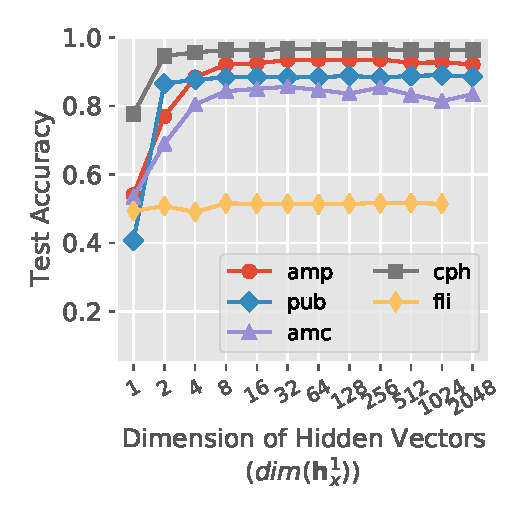
\includegraphics[width=0.4\columnwidth]{../figs/experiments/exp_hyperparameter_on_accuracy_gcn.pdf}}
        \subfloat[GGNN]{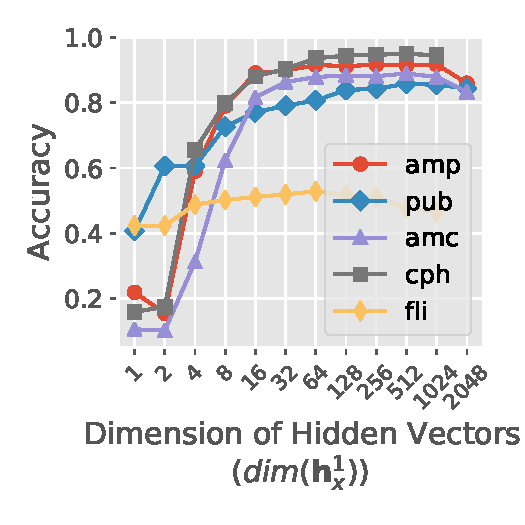
\includegraphics[width=0.4\columnwidth]{../figs/experiments/exp_hyperparameter_on_accuracy_ggnn.pdf}}\\
        \subfloat[GAT]{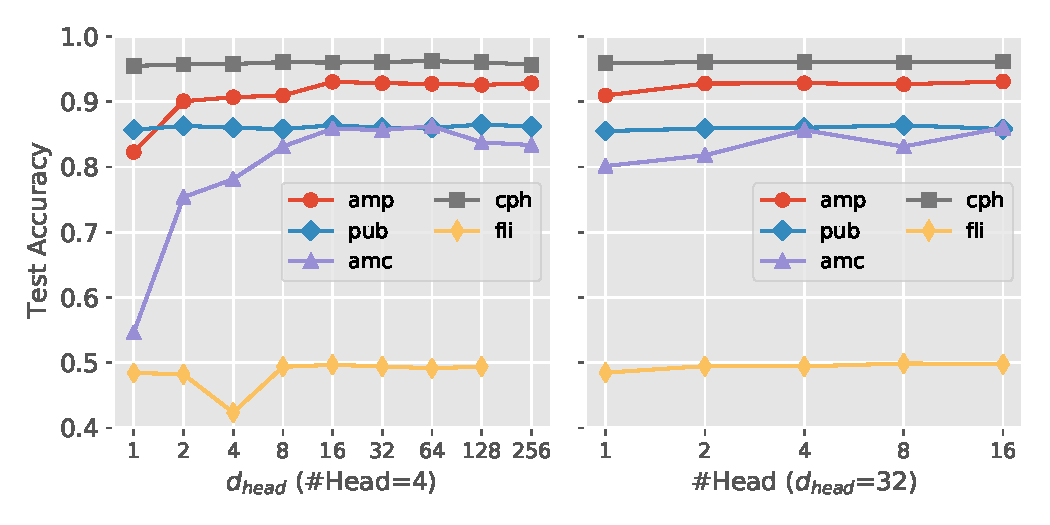
\includegraphics[width=0.8\columnwidth]{../figs/experiments/exp_hyperparameter_on_accuracy_gat.pdf}}\\
        \subfloat[GaAN]{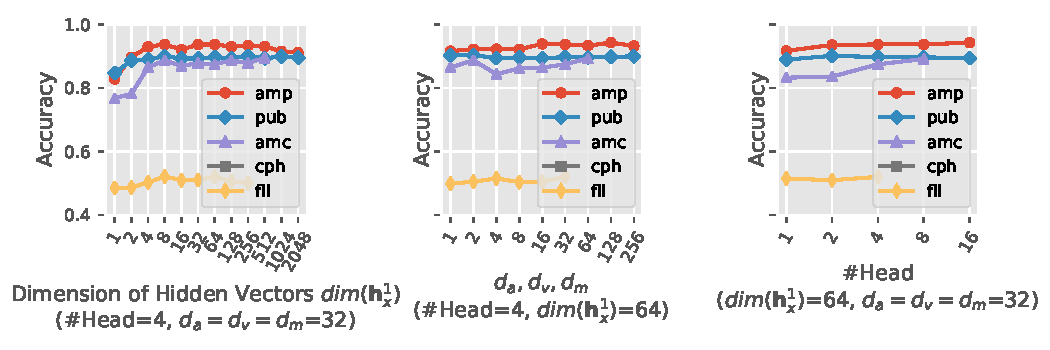
\includegraphics[width=1.0\columnwidth]{../figs/experiments/exp_hyperparameter_on_accuracy_gaan.pdf}}
        \caption{Effects of hyper-parameters on accuracy of the typical GNNs.}
        \label{fig:exp_hyperparameter_accuracy}
    \end{figure}
    
    %\begin{figure}[H]
        %\centering
        %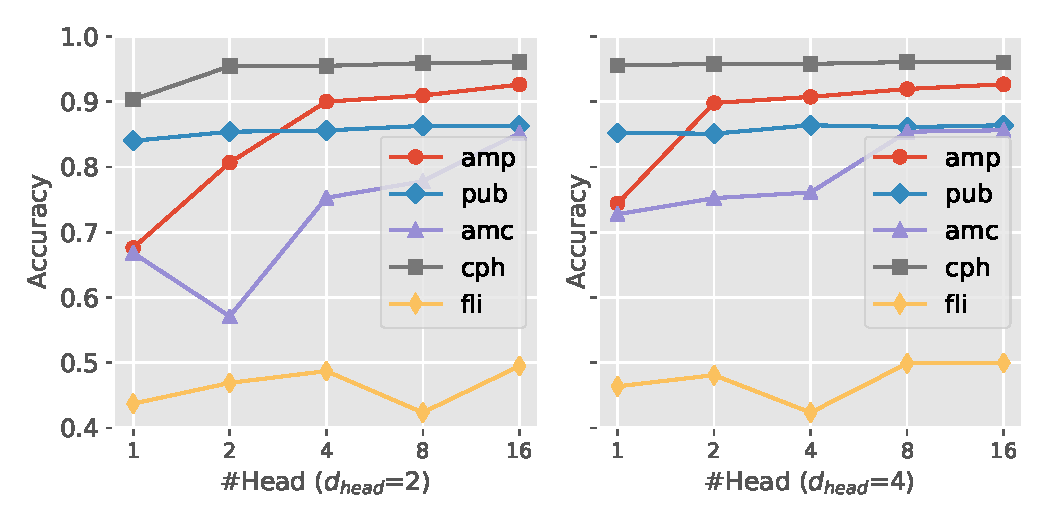
\includegraphics[width=0.5\columnwidth]{figs/experiments/exp_hyperparameter_on_accuracy_gat_small_info.pdf}
        %\caption{Effects of the number of heads on GAT ($d_{head}$=2,4)}
        %\label{fig:exp_hyperparameter_accuracy_gat_small_info}
    %\end{figure}
    
    \figurename~\ref{fig:exp_hyperparameter_on_accuracy_alg_contrast} (in the reply) further compares the best accuracy that each GNN could achieve on different datasets.
    %
    The best accuracy of the typical GNNs was very close.
    %
    %
    It was also close to the accuracy reported in their original references [34, 31].
    %
    The results indicated that there was no clear winner.
    %
    The relative accuracy between GNNs varied greatly with different datasets.
    %
    GaAN achieved the highest accuracy in three out of five datasets.
    %
    GCN achieved the highest or second highest accuracy in three out of five datasets, though its model was simplest.
    %
    Simple GNN models (such as GCN) could still achieve good accuracy with proper hyper-parameter settings.
    
    \begin{figure}[H]
        \centering
        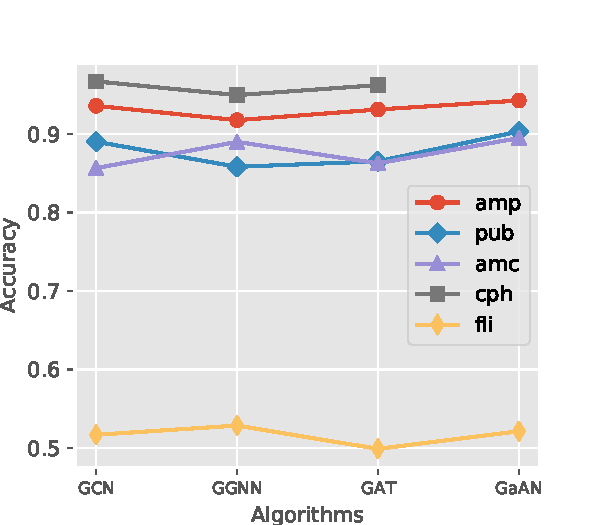
\includegraphics[width=3.5in]{../figs/experiments/exp_hyperparameter_on_accuracy_alg_contrast.pdf}
        \caption{Best accuracy that each GNN achieved on different datasets.}
        \label{fig:exp_hyperparameter_on_accuracy_alg_contrast}
    \end{figure}
    

    \end{myquote}
\end{reply}

\begin{point}
    Sampling method is definitely going to reduce model complexity, since all models complexity depend on graph node number N, while performance is going to be compromised as well. I would like to see authors resolve the concern of significant accuracy drop after applying aggressive sampling of subgraphs.
\end{point}

\begin{reply}

    Thanks for the insightful comment and valuable suggestion.
    %
    The sampling methods indeed affect the test accuracy of GNN models [5, 28, 26, 31].
    %
    Without sampling, the GNN models are trained with a \emph{batch} gradient descent manner.
    %
    With sampling, the GNN models are trained with \emph{mini-bach} stochastic gradient descent.
    %
    The structure of the GNN remains unchanged between batches.
    %
    Each GNN layer always consists of $|\mathcal{V}|$ graph neurons, where $|\mathcal{V}|$ is the number of vertices in the graph.
    %
    But the numbers of \emph{activated} graph neurons are different for different batches.
    %
    In each batch, only the neurons corresponding to the vertices appearing in the sampled subgraph will be activated.
    %
    The model parameters are updated according to the gradients calculated on the sampled subgraph in each batch.
    %
    Thus, the test accuracy of the models trained with sampling techniques may be different from the full-graph training.
    
    To discuss how the sampling techniques affect model accuracy, we have added a new subsection Section 4.2.2 ``Effects on Accuracy'' in Section 4.4 ``Effects of Sampling Techniques'' in the revised manuscript.
    %
    We quote from Section 4.4.2 of the revised manuscript to present our results.
    
    \begin{myquote}{Section 4.4.2 ``Effects on Accuracy''}
    
    Since the size of the sampled subgraph was much smaller than the original graph, the accuracy of the GNN models got by sampling techniques might be different from the full-batch training.
    %
    To find out how the batch size affected the test accuracy, we trained GNNs with different batch sizes.
    %
    \figurename~\ref{fig:exp_sampling_relative_batch_size_accuracy_graphsage} (in the reply) and \figurename~\ref{fig:exp_sampling_relative_batch_size_accuracy_cluster} (in the reply) compare the test accuracy achieved by sampling techniques with the test accuracy of the full-batch training.
    %
    For each combination of dataset and GNN, we chose the hyper-parameters that achieved the highest accuracy according to the experimental results in Section 4.1.
    
    \begin{figure}[H]
        \centering
        \subfloat[\texttt{amp}]{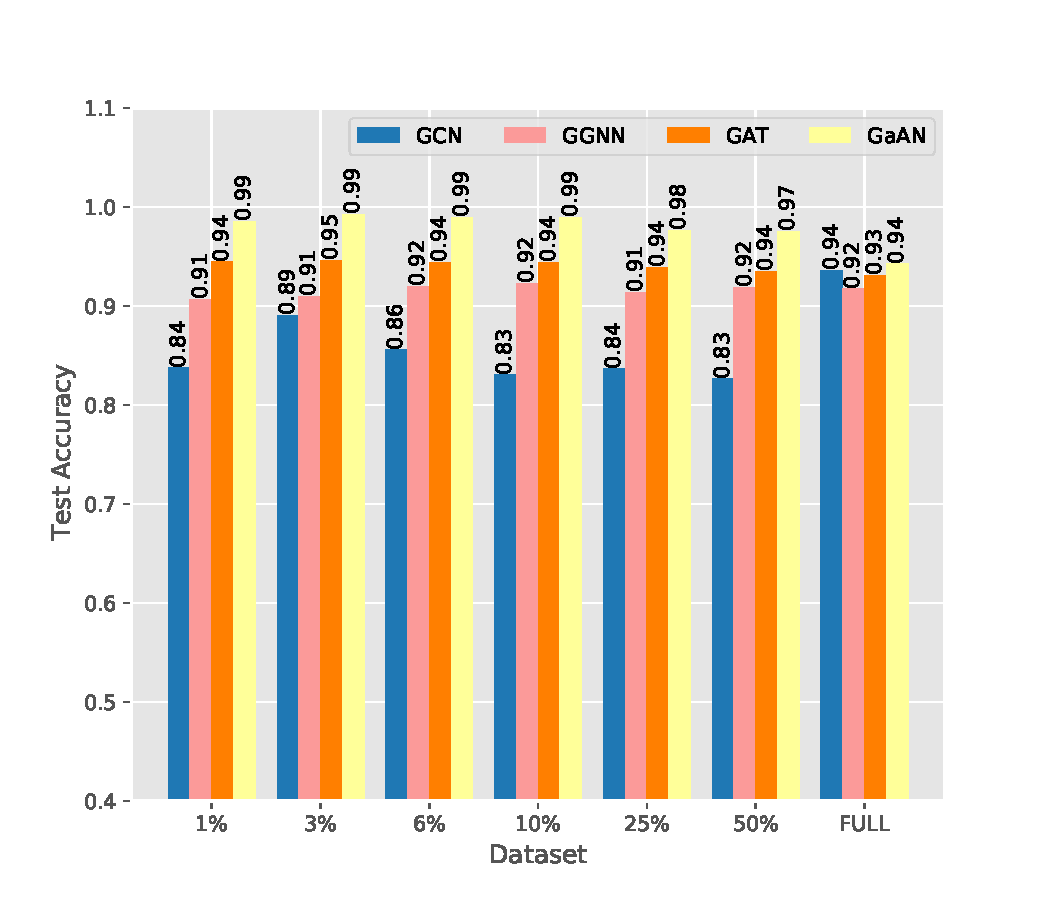
\includegraphics[width=2in]{../figs/experiments/exp_graphsage_sampling_accuracy_on_amp.pdf}}
        \subfloat[\texttt{amc}]{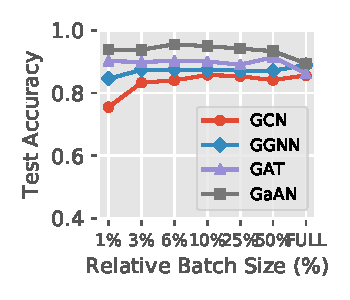
\includegraphics[width=2in]{../figs/experiments/exp_graphsage_sampling_accuracy_on_amc.pdf}}
        \subfloat[\texttt{fli}]{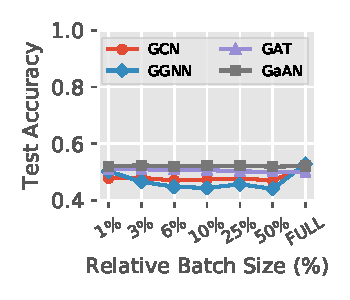
\includegraphics[width=2in]{../figs/experiments/exp_graphsage_sampling_accuracy_on_fli.pdf}}
        \caption{Test accuracy under different batch sizes of the neighbor sampler. FULL means that the full graph participated in the training.}
        \label{fig:exp_sampling_relative_batch_size_accuracy_graphsage}
    \end{figure}
    
    \begin{figure}[H]
        \centering
        \subfloat[\texttt{amp}\label{fig:exp_cluster_sampling_accuracy_on_amp}]{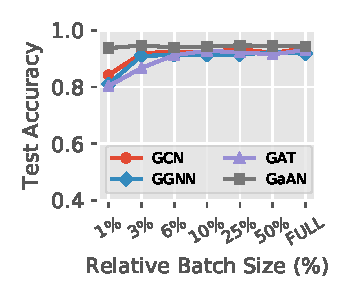
\includegraphics[width=2in]{../figs/experiments/exp_cluster_sampling_accuracy_on_amp.pdf}}
        %
        \subfloat[\texttt{amc}\label{fig:exp_cluster_sampling_accuracy_on_amc}]{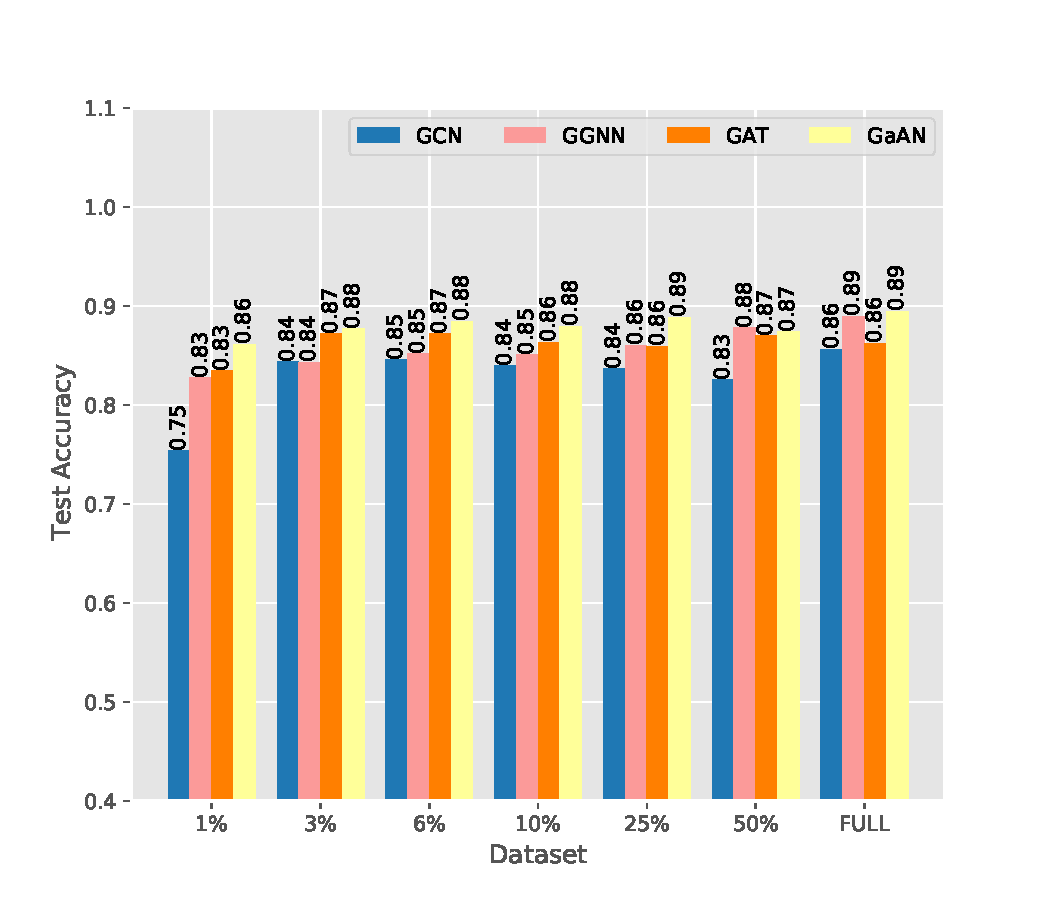
\includegraphics[width=2in]{../figs/experiments/exp_cluster_sampling_accuracy_on_amc.pdf}}
        %
        \subfloat[\texttt{fli}\label{fig:exp_cluster_sampling_accuracy_on_fli}]{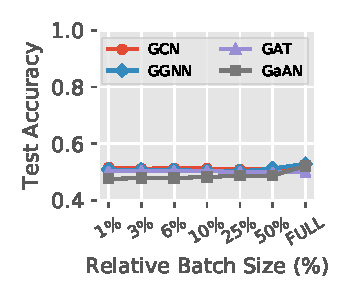
\includegraphics[width=2in]{../figs/experiments/exp_cluster_sampling_accuracy_on_fli.pdf}}
        \caption{Test accuracy under different batch sizes of the cluster sampler. FULL means that the full graph participated in the training.}
        \label{fig:exp_sampling_relative_batch_size_accuracy_cluster}
    \end{figure}
    
    The experimental results confirmed the effectiveness of the sampling methods in terms of accuracy.
    %
    When the relative batch size was greater than or equal to 3\%, the test accuracy of the GNNs trained with sampling was close to the accuracy obtained by full-batch training.
    %
    In most cases, the accuracy achieved by the sampling techniques was slightly lower than the full-batch training.
    %
    However, there were some exceptions (like GaAN in \figurename~\ref{fig:exp_cluster_sampling_accuracy_on_amp} and \figurename~\ref{fig:exp_cluster_sampling_accuracy_on_amc} in the reply) that the accuracy achieved by sampling was even higher.
    
    The relationships between batch size and test accuracy were complex.
    %
    A larger batch size did not always bring higher accuracy.
    %
    For example, the accuracy of GaAN in \figurename~\ref{fig:exp_cluster_sampling_accuracy_on_amp} (in the reply) and GGNN in \figurename~\ref{fig:exp_cluster_sampling_accuracy_on_fli} (in the reply) decreased as the batch size increased.
    %
    A smaller batch size sometimes could achieve higher accuracy.
    %
    For example, GAT achieved a higher accuracy with 1\% relative batch size than the full-batch training in \figurename~\ref{fig:exp_cluster_sampling_accuracy_on_amc} (in the reply).
    %
    Given a sampling method, we found that the optimal batch size highly depended on the dataset and the GNN algorithm.
    %
    Our observations were similar to [31].
    %
    How to automatically select a proper batch size is a topic worth further studying.
    
    Among the two sampling methods, the performance of the cluster sampler was stabler than the neighbor sampler.
    %
    With the cluster sampler, the test accuracy of different GNNs was very close to the accuracy of full-batch training.
    %
    With the neighbor sampler, the test accuracy of different GNNs showed more obvious differences.
    \end{myquote}
    
\end{reply}

\begin{point}
    Hope authors supplement the effect of sampling and GNNs on accuracy while comparing different complexity of model and sampling methods.
\end{point}

\begin{reply}

    We are grateful for your insightful suggestion.
    %
    As suggested, we additionally evaluated the effects of model complexity on accuracy in Section 4.1 ``Effects of Hyper-parameters on Performance'' in the revised manuscript.
    %
    We added experimental results on how the hyper-parameters of GNNs affected the accuracy.
    %
    Since different GNNs had different model complexity, we further compared the test accuracy of different GNNs on the same dataset.
    %
    More details are available in the reply to Reviewer Point P2.4.
    
    We also additionally evaluated the effects of sampling techniques on accuracy in Section 4.4 ``Effects of Sampling Techniques'' in the revised manuscript.
    %
    We presented the experimental results in a new subsection Section 4.4.2 ``Effects on Accuracy''.
    %
    More details are available in the reply to Reviewer Point P2.5.
\end{reply}

\end{document}